\documentclass[12pt]{ucalgthes1}
\usepackage[letterpaper,top=1in, bottom= 1in, left= 1in, right= 1in]{geometry}

\usepackage{natbib}
\usepackage{hyperref}
\usepackage{amsthm}
\usepackage{graphicx}
\usepackage{amsmath}

\bibliographystyle{abbrvnat}
\setcitestyle{authoryear,open={(},close={)}} %Citation-related commands

\graphicspath{ {./figures/} }
\usepackage{mathptmx}
\usepackage{mathtools} 
\title{Measuring Energetic Electron Precipitation using High Altitude Balloons and X-ray Spectroscopy\\ \bigskip
 }


\author{Matthew Patrick}
\thesisyear{2022}
\thesis{thesis}
\newcommand{\thesistitle}{Title of Thesis}
\monthname{February}
\dept{SPACE PHYSICS}
\degree{DOCTOR OF PHILOSOPHY}

\begin{document}
\makethesistitle
\pagenumbering{roman}     % resets page counter to one
\setcounter{page}{2}
%\chapter*{UNIVERSITY OF CALGARY \\ FACULTY OF GRADUATE STUDIES}
%\thispagestyle{empty}
%The undersigned certify that they have read, and recommend
%to the Faculty of Graduate Studies for acceptance, a \Thesis\ entitled
%``\thesistitle'' submitted by \Author\
%in partial fulfillment of the requirements for the degree of
%\Degree.\\

%
%                 Substitute  List of Examiners
%
%\begin{signing}{Department of Academic Computing}
%\signline
%Chairman, Dr.~John D.~Doe \\
%Department of Academic Computing \\
%Services  \\
%\signline
%Chairman, Dr.~John D.~Doe \\
%Department of Academic Computing \\
%Services  \\
%\signline
%Chairman, Dr.~John D.~Doe \\
%Department of Academic Computing \\
%Services  \\
%\signline
%Chairman, Dr.~John D.~Doe \\
%Department of Academic Computing \\
%Services  \\
%\newsigncolumn         use this command to start a new column if necessary
%\newsigncolumn
%\signline
%Chairman, Dr.~John D.~Doe \\
%Department of Academic Computing \\
%Services  \\
%\signline
%Dr.~Jane Smith \\
%Department of Academic Computing  \\

%\signline
%Dr.~A.~B.~Brown \\
%Department of Academic Computing  \\
%\end{signing}
%
\newpage
\phantomsection
\altchapter{\bf{Abstract}}

This work develops experimental methods to infer energetic electron precipitation using X-ray measurements from high altitude balloons. The problem of creating a mapping between the energies and fluxes of secondary X-ray radiation and the causative precipitating electron spectrum is solved using monte-carlo simulations and computer models of the detectors. The inverse problem of determining the electron spectrum from X-ray measurements is solved from first principles by treating the underlying ill-conditioning using regularization and preconditioning methods.  Validation using simulations of the precipitating electrons and detector demonstrates that the inverse problem is solvable for realistic experimental noise levels in the measured X-ray spectra. The problem of overfitting is solved using cross-validation techniques, which produces electron spectra that do not depend on assumptions about the amount of information that can be reliably determined from the experimental measurements.

X-ray spectrometer measurements from two University of Calgary high altitude balloon flights and a NASA BARREL balloon flight are analyzed using the developed methods. The resulting electron spectra are compared with the electron spectra obtained using conventional fitting techniques to show that exponential or mono-energetic models can under-fit the available data. A comparison between the BARREL balloon data and a magnetically connected RBSP measurement of the precipitating electron spectrum prior to scattering shows that the approximate energy range over which the applicable scattering processes in the radiation belts operate can be determined from the balloon data. The average electron flux measured from the balloon is shown to be consistent with the RBSP measurements under a strong scattering assumption. 

The combination of models produced using the developed analysis being consistent with previous experiments and correct based on simulated data is used to advance the case that balloon X-ray spectrometer measurements carry more information than is typically resolved using more simple techniques. 


\newpage
\phantomsection
\altchapter{\bf{Acknowledgements}}
Paragraph 1

Paragraph 2

Paragraph 3

\begin{singlespace}
\newpage
\phantomsection
\tableofcontents
\pagestyle{plain}
\newpage
\phantomsection
\listoftables
\pagestyle{plain}
\newpage
\phantomsection
\listoffigures
\pagestyle{plain}
\clearpage
\clearpage          
\end{singlespace}
\newpage
\phantomsection
\chapter*{\bf{List of Symbols, Abbreviations and Nomenclature}\hfill} \addcontentsline{toc}{chapter}{List of Symbols}
\listofsymbols
\pagestyle{plain}
\clearpage

\pagenumbering{arabic}
\chapter{Introduction}

\section{Like Astronomy, but Closer}

Space physics is a field of study that encompasses natural phenomena that occur in our own solar system. The basic difference between it, and the much older field of Astronomy is that in-situ measurements and direct experiments are possible. As a separate field of study, space physics began in earnest at the beginning of the space age with the flights of the first instrumented spacecraft. The discovery of the radiation belts that surround Earth was a profound example of the subsequently rapid increase in knowledge about the space surrounding Earth which is a trend that has continued to the present day. At the same time, and equally importantly, ground based and remote sensing techniques have advanced to the degree that robust, distributed, measurements of the properties of the space around Earth are readily available. The synthesis of these two orthogonal, but complimentary, sources of data gives the field of space physics a distinct image among the sciences, and motivates its pursuit not just for its own sake, but as a window to the workings of the wider universe which we cannot reach.

The space surrounding the Earth is full of activity. To get a picture of this, one can look at the Aurora Borealis, one of the dramatic and beautiful properties of this system. When they occur, the aurora aren't static features. Depending on the type of aurora, they can present as shimmering curtains, pulsing patches, or diffuse regions. These types are not exclusive. Dynamic structures like these, in space and time, are often indicative of a complex system. The old description - that the aurora are caused by the solar wind following the magnetic field of the Earth and hitting the atmosphere - falls flat in light of this complexity. In fact, the current state of knowledge paints a much different picture, with internal properties of the space and constituents surrounding Earth doing most of the ``work'' producing the aurora, which then carries much information about the entire system. 

There are two basic entities in near Earth space: fields and particles, which may be electrically charged. Classical electromagnetism provides a sufficiently accurate description of these in most cases. These are Maxwell's equations, in one of their most common forms:

  \begin{subequations}
    \begin{alignat}{2}
      \mathllap{\text{Gauss' Law}\qquad} && \nabla\cdot\mathbf{E} &= \frac{\rho}{\varepsilon_0} \\
      \mathllap{\text{Gauss' Law ($\mathbf{B}$ Fields)}\qquad} && \nabla\cdot\mathbf{B}  &= 0 \\
      \mathllap{\text{Faraday's Law}\qquad} && \nabla\times\mathbf{E} &= -\frac{\partial \mathbf{B}}{\partial t} \\
      \mathllap{\text{Ampere's Law}\qquad} && \nabla\times\mathbf{B} &= \mu_0\mathbf{J}+\mu_0\varepsilon_0\frac{\partial\mathbf{E}}{\partial t}
      \end{alignat}
        \end{subequations}

In these equations, $\mathbf{E}$ and $\mathbf{B}$ are the electric and magnetic fields, $\mathbf{J}$ is electrical current, $\rho$ is charge density, and $\mu_0 and \varepsilon_0$ are constants. These have been known for a long time, but they contain the root of why the space around Earth is a complicated place. When you have charged particles, they move according to electromagnetic fields, but while they move, they also affect the fields themselves. In an environment like near Earth space, where matter mostly exists as a plasma of charged particles, this gives rise to collective, or self-consistent behaviour and is a source of complexity. Further, a simple analysis of Maxwell's equations shows that wave phenomena also occur. This is combined with the fluid character that particles in large numbers display to make what is called plasma physics. 

Most of the matter in the space around Earth exists as a plasma. Plasma can be roughly defined as a gas of positive and negatively charged particles in approximately equal number, free to move, and at a high temperature. There is a more precise definition, which comes from statistical mechanics. In general, it is accurate to say that one of the defining characteristics of a plasma is the combination of the long-range electromagnetic wave interactions, with short-range collisional and fluid properties. Plasma waves, collective motion, and the propagation, absorption, and emission of radio waves are all observed in the space surrounding Earth. Based on all of this, the overall picture is not one of cold, dark, and empty space, but of a lively and energetic environment, constantly in motion and full of vibrations, with energy, matter, and information constantly flowing.

\begin{figure}[h]
\label{aurora_from_space}
\begin{centering}
\includegraphics[width=.5\textwidth,angle=270]{figures/chapter_1/aurora_from_space/aurora_from_space}
\caption{This picture of the Aurora, taken from the International Space Station, shows that the space around Earth can have a lively and energetic character. Image by NASA, from nasa.gov.}
\end{centering}
\end{figure}

The active transport of particles through the space around Earth motivates questions about their dynamics. One of the most basic questions is how constituent particles enter and leave the system. Understanding this is central to forming an accurate picture of the overall system. Experimental measurements are required to achieve this. The fact that the Aurora occur is evidence that some fraction of the particles in near-Earth space eventually end up in the atmosphere, where they deposit energy and create visible light. The fact that we can directly observe this secondary radiation makes it a compelling target for experimental measurements. The question then becomes what information about the original particles can be extracted from their impact on the atmosphere. This type of question is not uncommon in the physical sciences. An analogous problem in geophysics is the reconstruction of seismic events  from the vibrations caused at the surface of the Earth. This type of inverse problem naturally leads to a mismatch between the amount of data available and the amount required to generate unique solutions. In this thesis we address the problem of determining the population of electrons leaving geospace by impacting the atmosphere, using measurements of the secondary radiation they produce. Rather than visible light, the secondary X-rays produced by the electrons decelerating in the atmosphere are used as the source of data. 

The aim of this thesis is to develop the techniques necessary to obtain useful information from this indirect measurement. The combination of practical problems due to the need to obtain measurements at high altitudes of greater than 30 kilometers or so, and the mathematical problem of reconstructing useful models from incomplete secondary data lead to a challenging experiment. We show that a surprising amount of detail about the particles in geospace can be found despite these challenges.

\section{The Earth's Atmosphere and Geospace}

The experiments described in this thesis are conducted within the Earth's upper atmosphere, with detectors carried onboard stratospheric balloons. The processes that these experiments measure occur on the boundary between space and the atmosphere.  An accurate description of this region is therefore needed to analyze data from the experiments. 

At the surface of the Earth, the atmospheric constituents are well-mixed. Most of the mass of the atmosphere lies in the region defined as the troposphere, which extends from ground level to to an altitude of around 10 kilometers. This dense region of the atmosphere is where life on Earth, and most terrestrial weather happens. The main structure of the troposphere is defined by a decrease in temperature and density with increasing height. Density decreases exponentially with altitude, which can be shown from the hydrostatic condition. Temperature is somewhat more complicated. Besides local effects (weather), temperature decreasing with height owing to the decreased gravitational potential. The lapse rate defines the rate at which temperature drops with height, and has a value of approximately $2^{\circ}$  C per kilometer of altitude. 

At the tropopause, the temperature of the atmosphere begins to increase with height. The density here is low enough that ultraviolet radiation penetrates and causes the disassociation of molecular oxygen, which results in free oxygen atoms combining with diatomic oxygen to form ozone. The stratosphere is characterized by limited vertical mixing, and is very dry, with few weather effects from the troposphere reaching it. Winds in the stratosphere can be intense, reaching speeds of hundreds of 200 kilometers per hour. This presents interesting operational challenges to experiments carried on balloons in this region, particularly with regards to their post-flight recovery. 

The density in the stratosphere is low, ranging from a few percent of that at ground level to nearly zero at the vertical limit. The low density in the stratosphere makes it quite transparent to certain kinds of radiation from space. In particular, X-rays, created from the slowing down of charged particles farther up in the atmosphere, can propagate deeply in this region. This is where remote sensing of space effects based on secondary radiation becomes possible using balloon-borne instruments, which are discussed in the following section. 

At the end of the stratosphere, temperature once again begins to decrease with height. This occurs at an altitude of approximately 50 kilometers above the surface of the Earth. The mesosphere is the name given to this region of the atmosphere. Here, the different components of the atmosphere are still well-mixed owing to turbulence. This continues to be true to a height of around 80 kilometers. Meteorites burn up in this part of the atmosphere, and the temperature reaches a lower limit of approximately -100 degrees C at its highest point. Once the turbulent effects which occur in the mesosphere become less important, separation of the different atmospheric constituents occurs due to the different scales at which their densities decrease. The hydrostatic condition imposes exponential decreases in density with height, but the scale at which this happens depends on the particle mass. This gives rise to a structure in the upper atmosphere, with the proportions of the different components changes with height. This is important for modelling the propagation of  radiation, which has interactions which depend on the chemical composition, overall density, and temperature. 

Past the mesosphere lies a region called the thermosphere. In this region, temperatures climb sharply and then are steady with increasing height. Solar activity has a strong bearing on the temperatures in this region, which can reach hundreds or thousands of degrees C. Turbulant mixing no longer has meaning at the low densities in the thermosphere. The international definition of the beginning of space, a boundary that begins at 100 kilometers altitude, is contained in this region. In the thermosphere, the density begins to become sufficiently low that the rate of collisions between individual atoms and molecules becomes small enough to start treating them individually, rather than as a fluid. This is the domain where plasmas can exist, since ionized particles and electrons do not immediately collide and become neutral once they are created. This region of space overlaps with the ionosphere, for this reason.  Spacecraft orbit in the thermosphere; orbits with a practical decay time begin at heights of around 350 kilometers.

At heights of hundreds of kilometers, charged particles survive for long enough that electromagnetic interactions become important. Temperature takes on a different intuitive meaning, one based more on the statistical properties of individual and group particle motion, then the classical value that can be measured with a thermometer. The local magnetic field becomes the most important geometry and coordinate system, rather than the local vertical direction from Earth. Free from the dominating effect of collisions, particles undergo characteristic motions not seen in the lower regions of the atmosphere, which are determined by electric and magnetic fields. Figure~\ref{atmosphere_schematic} shows an illustration of some the different layers of the atmosphere, and how the population of charged particles changes with height.

It's not easy to draw a clear sharp line where the atmosphere ends. Such a definition probably needs to depend on the application or line of inquiry being pursued. For aircraft, heights past the stratosphere are unreachable owing to low density. Rockets can reach the intermediate heights between the stratosphere and the thermosphere, while orbiting satellites require further heights still, so that orbits decay on a sufficiently large timescale. Eventually, even the magnetic field of the Earth becomes less important than the magnetic field carried with the plasma of the solar wind, and farther past this point, the influence of the Earth and its magnetic field ceases. The exploration of the solar system, and beyond, by robotic spacecraft begins to  blur the distinction between space physics and astronomy. It is interesting, that the two fields are separated mostly by a practical limitation due to the vast distances involved, instead of a more fundamental, and natural boundary.


\begin{figure}[p]
\label{}
\begin{centering}
\includegraphics[width=.9\textwidth]{figures/chapter_1/atmosphere_schematic/atmosphere_schematic}
\caption{Schematic illustration showing the scale and structure of the atmosphere, with the overall trend in electron density with height. Image by NASA Goddard, from nasa.gov.}
\end{centering}
\end{figure}
\newpage

\section{Getting Above the Atmosphere with High Altitude Balloons}

Since the atmosphere shields most of the radiation from space, it is not possible to build ground-based experiments that are sensitive to X-ray and charged particle radiation. Rocket flights routinely reach heights where this is no longer a problem, but by their nature, the flight times are short, on the scale of minutes. Orbiting satellites are practical at altitudes far above where radiation from space deposits most of its energy, so there needs to be another kind of vehicle, to get instruments above most of the atmosphere by mass, and that can remain there for hours, or days. Balloons provide data which are distinct from satellites. In the types of balloon experiment conducted in this thesis, radiation detectors are designed with a field of view that extends above them and covers a circle in the sky. The detectors measure secondary radiation produced by energetic particles which enter the atmosphere. On the other hand, satellites do measurements along the path of their orbit, and see particles that have not entered the atmosphere. Additionally, balloons move slowly compared to satellites, and can therefore accomplish measurements of roughly the same region over extended periods.  

Balloons are the vehicles used in this thesis to get above the shielding effects of the lower atmosphere, and measure radiation from space directly at an altitude of 30 to 40 kilometers. High altitude balloons are large, thin, membrane structures, filled with either hydrogen or helium, which carry payloads ranging from grams to hundreds of kilograms, and ascend until they reach an equillibrium height in the stratosphere, above most of the radiation shielding effects of the atmosphere. Balloons need no external energy source to maintain their flight, and so can remain at altitude for hours, days, or even weeks depending on their design and the desired mission profile. With the exception of the balloons needed to carry the largest, heaviest, experiments, high altitude balloons are also inexpensive, compared with rocket flights and satellites. This opens possibilities for extensive surveys and coincident missions which do not exist when using other platforms. 

High altitude balloons follow two distinct designs. The zero-pressure balloon is  named because it maintains an internal pressure equal to the surrounding atmosphere. This is the type of balloon most frequently used for scientific experiments, because it has the property of passively remaining at peak altitude for extended periods of time. The design consists of a large polyethelyne bubble, with one or two vent ducts near the bottom, which are open to the atmosphere. The payload hangs beneath the balloon on a cable or rope. As the balloon is filled through the ducts, lift gas collects at the apex and causes hydrostatic lift. Once a predetermined amount of lift gas has been added, the balloon is released, and ascends, carrying the payload with it. As the balloon ascends, the internal lift gas expands to fill the balloon volume. Eventually, the balloon is completely filled with the low density lift gas, and excess is passively released through the vent ducts, causing the balloon to stop ascending and maintain a fixed altitude. When the balloon mission is terminated, cable cutting equipment is used to separate the payload from the balloon. The payload descends under parachute and is usually recovered. Upon release of the payload, it is typical that the payload rips a destruct panel from the balloon, causing it to release most of its lift gas and descend as well. The point at which the termination process happens is chosen in the design phase of the mission, and can be activated by timer, remote command, or both. 

There is an ultimate limit to the flight duration which can be achieved using zero-pressure balloons, which is caused by internal temperature differences at day and night. During the day, solar radiation warms the balloon and the gas contained in it. When night occurs, the balloon begins to cool, which causes the gas inside to decrease in volume. The balloon has no rigid structure to maintain a fixed volume, so the balloon membrane then occupies less volume as well. This causes the balloon to start to descend, where it reaches a new equillibrium point. At sunrise, solar heating causes the balloon to rise again, although it will not reach the same altitude it started with. For long duration scientific experiments, this  cycle is controlled  through the release of ballast, usually sand. It can be shown that the ultimate limit for the duration of zero pressure balloon flights is approximately 7 days, even if most of the payload consists of expendable ballast. The exception to this rule occurs for flights in the polar regions of the Earth, where the day night cycle is longer. Figure~\ref{zero_pressure_balloon_example} shows a zero-pressure balloon in flight, with the scientific payload being carried below.

\begin{figure}[p]
\label{zero_pressure_balloon_example}
\begin{centering}
\includegraphics[width=.7\textwidth,angle=270]{figures/chapter_1/zero_pressure_example/zero_pressure_example}
\caption{Zero-pressure balloon in flight shortly after release. The lift gas will expand to fill the balloon volume during the ascent.}
\end{centering}
\end{figure}
\newpage

The second type of high altitude balloon is primarily used for meteorological experiments. Consisting of a relatively small latex sphere, this balloon is closed from the atmosphere and rises until the internal pressure causes it to rupture and descend. These meteorological balloons are launched regularly around the world several times per day to aid in the creation of weather models and forecasts. Typically carrying payloads of only a few hundreds of grams, to at most a few kilograms, these balloons reach heights comparable to the zero-pressure balloons, but do not maintain equillibrium altitude. This makes them less useful for the measurement of space radiation, although, some exotic ways to overcome this problem have been developed and tested.


\section{Scope of this Thesis}

The question is: what is the maximum amount of information that can be obtained about processes far out in the space surrounding Earth, using measurements of the resulting radiation, and what kinds of instruments do we need to use to get the requisite data? This question is interesting because the experiments take place on the boundary between what we can directly affect using active experiments, and what we only learn through passive observation. Right now, most experimentalists are earth-bound, and this is unlikely to change in the near future. On the other hand, the types of experiments we fly on high altitude balloons provide a window to the wider universe, in a way that, unlike orbiting spacecraft, which require years or decades of planning, can be rapidly iterated on and repeated. The upper atmosphere can be thought of as a giant laboratory, and a detector which is sensitive to the radiation incident upon it from space. We have the ability to send experiments to this region rapidly and at low comparative cost to spacecraft. There is therefore a scientific return on being able to maximize the information we obtain from these experiments. The problem of mapping the available measurements of secondary radiation back to the particles impacting the atmosphere is required for this to happen. The following chapters will show the development of a solution which can be used to increase the observational power of balloon-borne experiments.

 



\chapter{Energetic Electron Precipitation and Geospace}

\section{Introduction to Connected Geospace}

The Earth is a complicated place. Natural processes, which occur on vastly different time scales, are all connected to each other and produce the state of the overall system. Only in the last 70 years or so, since the beginning of the space age, has the picture of the Earth as a dynamic system been extended to include the space around it. This space is not empty, and it has structure and dynamics which are very different than processes on Earth, mostly owing to the importance of the electromagnetic force between its constituents. The word used to describe the space around Earth is geospace, so-named because the Earth and its processses are not strictly separated from the space around it. In fact, information, matter, and energy flow between regions which can be separated by great distances, and cause effects which can echo throughout the entire system. In this chapter, we will describe one of the most dramatic ways which this can happen, where energetic particles from space enter the atmosphere and affect it directly. 

Energetic electron precipitation is a process by which electrons depart trapped states in geospace and enter the Earths atmosphere. One of the most brilliant effects that can be caused by this process is able to be seen from the ground on Earth - the northern lights, or Aurora Borealis. There has been a great deal of work done in the last half-century to understand, quantity, and model the processes responsible for creating the Aurroa, but many unanswered questions remain. With the knowledge that the Earth and the space around it are both connected and affect each other, it becomes of great scientific interest to understand the ways which particles and energy move between them. The fact that energetic particle precipitation can have dramatic visual affects on the atmosphere motivates its use as measurable target which can provide a window to the dynamics of the connected system. 

The earth and geospace are not stationary systems. One can draw a loose analogy between their related structure and the anatomy of a living organism. While the system is always in a state of change, there is a consistent structure and organization at the highest levels. In this case, that structure is largely defined by the magnetic field of the Earth, and the magnetic field of the solar wind which interacts with it. Navigation on the surface of the Earth can be accomplished by measuring the direction of the local magnetic field in two dimensions. In geospace, the magnetic field changes significantly over all three dimensions, and, to an extent, in time as well. As charged particles, electrons in geospace are subject to the Lorentz force. This force is always orthogonal to the magnetic field, which is why the magnetic field is such a powerful organizational force in the system. 

The magnetic field of the Earth is due to both internal, and external (space-based) current sources. This field can be conveniently described by the multipole expansion. Figure~\ref{magnetosphere_diagram} shows a model of the magnetic field of the Earth, which takes into account both internal and external sources. Towards the surface, the dipole is a fairly good fairly good approximation. Farther away, however, higher-order terms become important and result in a field has a vastly different structure than the dipole description, on scales which exceed around one Earth radius. The magnetic field geometry in Figure~\ref{magnetosphere_diagram} does not imply a steady-state to the system. Rather, this can be thought of as the overall topology of a system which is always in motion. In reality, only some modified version of this picture will be accurate at any particular time. Particularly, at distances which exceed a few Earth radii, the state of the solar wind, through which the Earth is always moving, becomes more important than the current sources internal to the Earth itself. A more accurate picture of the system than Figure~\ref{magnetosphere_diagram} would actually be an animation, with magnetic field lines cascading on the dipole field of the Earth, and reconnecting to form the stretched-out ``tail'' from 10 to hundreds of Earth radii ``downwind''. The description of that process is an entire field of study, and it too, has questions which are currently unanswered.

\begin{figure}[p]
\label{magnetosphere_diagram}
\centering
\includegraphics[width=1.1\textwidth,angle=180]{figures/chapter_2/magnetosphere_diagram/magnetosphere_diagram}
\caption{Model of the magnetic field of the Earth which includes effects due to external sources and the solar wind. Coordinates are measured in Earth radii and centered on the Earth. Near to the earth, a dipole field describes the geometry well. Farther away, this changes. }
\end{figure}

The simplistic view is: given that electrons in geospace exist, and they are subject to a magnetic field geometry which is complicated and dynamic on the relevant scales, this suggests that the motion of electrons within the system is important to the state of the overall system. This, then, implies that the loss of these particles to the Earths atmosphere, is also important. The goal of this chapter is to describe, in adequate detail, the connection between the precipitation of electrons into the atmosphere and the state of the larger geophysical system. The goal is to advance electron precipitation, which is a fairly dramatic event, as a process which is both worth understanding in its own right, but also as a tool, which provides a window in to the processes which occur in the larger system. 

\section{Electrons in Geospace}

The first American artificial satellite, Explorer 1, was launched in 1958. Among other instruments, it carried a Geiger counter, which is a device sensitive to the energy deposition of charged particles like electrons. The expected background count rate due to cosmic rays was observed at some points during the flight, but at others, zero counts were reported. This was determined on later flights, to be due to the saturation of the device by a much larger than expected radiation flux. This led to the discovery of the radiation belts around the Earth. The question then became why the radiation belts existed, and what their properties are. A review of the historical development of knowledge about the radiation belts is~\cite{baker2012}. 

The radiation belts have a spatial structure. This is shown in Figure~\ref{radbelts_structure}, which is an evaluation of a fairly standard model, AE9, see~\cite{ginet2013}. An approximate description of the Earths magnetic field is overlaid to show that the it is the main geometry at play. There are three essential regions. The inner zone, and outer zone are distinct and separated by a region of empty space, called the slot region, in between them. The development of knowledge of how the radiation belts are formed took longer than knowledge about their essential spatial structure, which we will summarize. 

\begin{figure}[p]
\label{radbelts_structure}
\centering
\includegraphics[width=1.0\textwidth,angle=180]{figures/chapter_2/radbelts_structure/radmodel}
\caption{Cutaway view of model electron fluxes in the radiation belts, with some magnetic field lines to show the overall geometry.}
\end{figure}

The main process which is thought to be responsible, at least partially, for the existsnce of the inner radiation belt is called cosmic ray albedo neutron decay (CRAND)~\citep{singer1958}. In the CRAND process, cosmic rays from space create neutrons in the upper atmosphere, which are then free to travel upwards, or downwards. Those which travel upwards, and subsequently decay into a proton and an electron, form the inner radiation belt. Although one might be tempted to look to direct trapping of cosmic ray particles in the Earth’s magnetic field as a source instead of CRAND, which is a secondary effect, it has been shown that sources like this are not sufficient to explain the number and energies of particles in the inner radiation belt~\citet{hess1960}. 
Despite the fact that the CRAND process provides an explanation for the distribution of particles in the inner radiation belt [Farley et al., 1970], there are still some deficiencies that are not yet resolved. Because the CRAND process can only produce electrons up to 780 keV~\citet{baker2012}, it must be combined with some as-yet undetermined acceleration mechanism to explain observations of particles up to the 1 MeV range, which have been published as early as~\cite{hess1962}. With the exception of the unknown acceleration process, the current state of knowledge of the ultimate origin of particles in the inner radiation belt is essentially a combination of the trapping of solar wind particles, radial diffusion from the outer radiation belt, and the CRAND mechanism.

The gap that defines the separation of the inner and outer radiation belts is called the slot region, and is caused by a kind of radio wave called a “whistler” that is produced naturally by lightning on Earth~\citet{thorne1973}. As the radio wave interacts with particles trapped in the slot region it changes their motion in such a way that they fall out of their orbits to be lost in the Earth’s atmosphere. This process can be partially understood through the adiabatic description of trapped particle motion, which is discussed in Section ??. Even though steady-state and adiabatic expressions of the process by which the slot region is formed make predictions that agree with experimental data, they do not form a complete description. 

The outer radiation belt is very different in energy and spatial structure than the inner radiation belt. Besides being physically farther away from the Earth than the inner radiation belt, the outer radiation belt proton flux is much greater.\cite{hess1965} argues that since the neutron albedo is smaller farther away from the Earth, but despite this the proton intensity in the outer radiation belt is higher, CRAND cannot be the explanation for the existence of particles in this region. There were some competing ideas about the ultimate source of particles in the outer radiation belt, but it is currently believed that the source is some currently unknown mechanism which accelerates magnetospheric particles to relativistic speeds on hour-long time scales~\citet{baker2012}.

 \section{Single Particle Motion}
 
 Some properties of the radiation belts, and electron precipitation, can be understood through a simplified picture of their dynamics which considers particles independently. In this description, particle motions do not affect each other, that is, we ignore the fact that a charged particle moving an an electromagnetic field also creates an electromagnetic field due to its own motion. This picture neglects the collective effects characteristic of space plasmas. As a simplified picture, though, it provides a useful framework in which to describe the mechanism and effects of particle loss to the atmosphere.

For the purposes of this description, electrons from the radiation belts are free to move under the influence of the Earths magnetic field. The Lorentz force, $\mathbf{F} = q(\mathbf{v}\times\mathbf{B})$, where $q$ is the electron charge, $\mathbf{v}$ is the velocity vector, and $\mathbf{B}$ is the static magnetic field, is the only force which they are subjected to. This causes cycloidal motion about magnetic field lines. There is no component of the force parallel to the magnetic field, so the electron is trapped, to orbit the field line and drift along it at whatever parallel velocity it started with. 

There is a framework which is very useful in describing this kind of motion. If we consider a phase-space, where the momentum of the particle $P$ is along one axis, and the spatial coordinate $q$ is along another, then, under slow changes to the path integral:

$$\oint P dq$$

compared to the periodicity of the system, there will be an approximately constant quantity. This quantity is called an adiabatic invariant. For electron gyro motion around a magnetic field line, the associated invariant is:

$$J_1 = \frac{m v_{\perp}^2}{2B}$$

where m is the electron mass, $v_{\perp}$ is the electron speed perpendicular to the magnetic field, and B is the local magnetic field strength. Since the electron gyro frequency is fast (order of Mhz), this is a well conserved quantity, until one considers scattering by wave phenomena. In the situation where scattering is not occurring, electrons will increase their gyro frequency as they enter regions of space with increasing magnetic field strength, such as occurrs towards the magnetic poles of the Earth. The fact that the magnetic force does not do work has an important implication. When the gyro frequency of the particle increases, the component of the velocity which is parallel to the magnetic field decreases, to conserve the overall kinetic energy. Eventually, the electron can reach a point where all of the kinetic energy is due to the perpendicular component of the velocity. This will prevent the electron from going further into the intensifying magnetic field strength, and it will turn around, and mirror, heading in the opposite direction. Define the pitch angle, $\alpha$ as the angle between the electron velocity vector and the local magnetic field. If $B_0$ is the magnetic field strength at the equator, and $b_m$ is the local magnetic field strength, then the pitch angle is:

$$\sin^2\alpha = B_0/B_m.$$

This is the first-order, simplified picture of how electrons move in the near-Earth space environment. The electrons undergo gyro motion about magnetic field lines, and due to the invarant $J_1$, they bounce between the magnetic poles in (relatively) consistent orbits. This is called magnetic mirroring, and is possible due to the near-field approximation of the Earth's magnetic field as a dipole, where magnetic field strength increases towards the poles. Particles with motion nearly parallel to the magnetic field lines avoid this processes, and are lost to the atmosphere. The set of pitch angles for which electrons fail to mirror and enter the atmosphere is called the loss cone. When particles are scattered to pitch angles which fall into this loss cone, they precipitate, and are lost to the atmosphere. 

The bounce-motion of electrons between hemispheres is itself, periodic motion, and gives rise to another approximately conserved quantity. Choose the momentum coordinate to the along the magnetic field line with distance element $ds$, and the momentum to be the parallel component $mv_{\parallel}$. The associated invariant is then:

$$J_2 = \oint v_{\parralel}ds$$

for mirror-trapped electrons. The bounce time between mirror points for electrons in geospace is on the order of a few seconds, so this is a fairly well-conserved quantity for processes that occur on any time scales longer than that. This has another implication for particle motion in the radiation belts. Since the magnetic field in geospace is not a perfectly symmetric dipole, there is a-priori expectation that a bounce-trapped particle should return to the same mirror point between bounces. However, because the field is actually asymmetric, travel between different mirror points would imply a different path length in $J_2$. Since this is an approximately conserved quantity, electrons will oscillate between approximately the same mirror points on each bounce, even when the magnetic field they travel through is not symmetric or uniform.

\section{Scattering Processes}

Single particle motion describes a picture of the radiation belts which accounts for their overall anatomy and steady-state behaviour. This picture changes when dynamic effects occur that cause particles to leave the system and precipitate to the atmosphere. In this section, we will give a high level description of how and why these processes occur, and what some of their known effects are. The emphasis will be on how these processes connect to the larger picture of geospace, rather than the details of the physics governing each one. We advance the idea that, as both a cause and a result of processes in the magnetosphere, electron precipitation is an important feature of geospace, and needs to be understood to have an accurate picture of the entire system. 

Following the survey by~\cite{Millan2007a}, we can trace the development of knowledge of energetic electron precipitation from~\cite{Bailey1968}, who inferred the process by observing daytime decrease of forward scatter radio signals. \cite{rosenberg1972} used changes in the scattering of VHF radio signals to determine folding energies of 100 to 150 keV for observed electron precipitation. Subsequently,~\cite{parks1979} used balloon measurements of X-ray bremsstrahlung at energies of greater than 150 keV to infer precipitation. The first comtemporary review of balloon-borne measurements of energetic particle precipitation was given by~\cite{parks1993}. Balloon-based measurements of energetic electron precipitation now have an extensive heritage, and are one of the standard tools for measuring its effects. 

Broadly speaking, there are two main ways which electrons can be lost from the radiation belts: pitch angle scattering, due to interactions with radio and plasma waves, and radial diffusion outwards to the magnetopause~\citep{cao2017}. We will focus on pitch angle scattering, because it is this process which results in electron precipitation to the atmosphere. \cite{Millan2007a} present an overview of the current state of knowledge, which began with work done in the 1960s and 1970s, showing that wave-particle interactions can lead to pitch angle scattering and subsequent loss to the atmosphere~\citep{kennel1966, thorne1971, thorne1974}. Pitch angle scattering is a process where charged particles interact with wave phenomena, altering their pitch angles. When particle pitch angles are changed to fall into the loss cone, precipitation will occur. 

Wave-particle interactions perturb the natural coordinate system for charged particles in the radiation belts. When a wave phenomenon has a doppler-shifted frequency $\omega$ which is resonant with the relativistic electron gyrofrequency. This condition is written as:

$$\omega - k_{\parallel}v_{\parallel} = \frac{n\Omega_e}{\gamma}$$

where $k_{\parallel}$ and $v_{\parallel}$ are the parallel components of the wave vector, n is an integer multiple, $\gamma$ is the relativistic factor, and $\Omega_e$ is the electron cyclotron frequency. When these resonant interactions occur, energy and momentum are exchanged between the wave and the electrons. \cite{schulz1974} developed a quasi-linear framework which can be used to quantify this interaction. The partial-differential equation expresses the change in particle phase space density in a bounce-motion averaged sense, and depends on diffusion coefficients which need to be specified for the interacting plasma wave, using a model. 

There are three main types of wave which are responsible for causing pitch angle scattering and electron precipitation. The first two we will discuss, plasmaspheric hiss, and whistler chorus, are different manifestations of the same type of wave propagation, called whistler-mode. Whistlers were named by world war one radio operators, who would hear them on radio receivers. While they are radio waves, their frequencies occur over the audio range. The name comes from the fact that the received tone decreases in frequency over a time scale of a few seconds. 

\subsection{Whistler Mode Waves}

Whistler-mode radio waves are right hand circularly polarized waves which occur over the very low frequency (VLF) radio range, from approximately 3 to 30 Khz. Whistlers have frequencies in the audio range, so detection is fairly simple, and can be accomplished using a sensitive audio amplifier and a long (several meters) wire antenna. The special property which makes whisters interesting in the context of the radiation belts is that their dispersion relation causes them to propagate roughly along the magnetic field lines of the Earth, and subsequently bounce between magnetically conjugate points. Since the whistler waves travel thousands of kilometers out into the radiation belts and the magnetosphere, they carry back information about the state of these systems~\citep{ratcliffe66}. This is what motivated some of the early work in understanding whistler mode propagation. 

Whistlers are understood to be the result of lightning strikes which happen on Earth. When a lightning strike occurs, it creates a pulse of radio waves which travel to the ionosphere at roughly the speed of light, before entering what is called the earth-ionosphere waveguide~\cite{ratcliffe66}. The magnetized plasma in the ionosphere and out into the magnetosphere results in a particular dispersion relation and effective refractive index for the radio waves, which causes their unique behaviour. As the wave propagates through space, its frequency will change, producing the characteristic chirping sound. The waves may bounce between magnetically conjugate points several times, and when there are many of them, make sounds together that sound almost musical. 

The dispersion relation for whistler mode propagation determines how the frequency $\omega$, is related to the wavenumber $k$, of the whistler mode waves. The derivation is accomplished using the theory of radio propagation through cold plasmas and several approximations, and results in the relation:

$$\frac{c^2k^2}{\omega^2} = 1 - \frac{{\omega_{pe}}^2}{\omega(\omega - |\Omega_e|)},

where $c$ is the speed of light, $k$ and $\omega$ are the is the wave number and frequency of the radio wave, $\omega_{pe}$ is the electron plasma frequency, and $\Omega_e$ is the electron gyro frequency. The plasma frequency $\omega_{pe}$ is given by:

$$\omega_{pe} = \sqrt{4\pi N e^2/m}$$

where $N$ is the electron number density, $e$ is the electron charge, and $m$ is the electron mass. The plasma frequency can be thought of as a natural frequency which the positive and negatively charged components of the plasma would oscillate at if there were separated by some small distance and released. 

\begin{figure}[p]
\label{whistler_spectrogram}
\centering
\includegraphics[width=1.0\textwidth,angle=0]{figures/chapter_2/whistler/Whistler_radio_palmer_2004-07-23_T035528.png}
\caption{Frequency/time relation for a typical whislter wave, observed by a Stanford University VLF radio receiver at Palmer Station, Antarctica.}
\end{figure}

A spectrogram showing how a typical whistler wave changes frequency in time is contained in Figure~\ref{whistler_spectrogram}, reproduced from data by the Stanford University VLF group. The radio receiver used to record these data were located at Palmer Station, Antarctica. The characteristic chirp decreasing in frequency is apparent. 

\subsection{Plasmaspheric Hiss}

Plasmaspheric hiss is a particular kind of whistler-mode wave which is responsible for the formation of the slot region in the radiation belts~\citep{lyons1972, lyons1973}. The frequency range is broadband ELF, occupying 100 Hz to a few KHz~\citep{millan2007}. The generation mechanism is not fully understood. Unlike whistler waves, plasmaspheric hiss shows no relation to lightning strikes at frequencies below 1 Khz~\citep{meredith04}. Theoretical modelling is consistent with generation by the electron cyclotron instability~\citep{millan2007, huang1983, church1983, meredith04}. The electron cyclotron instability, described by~\cite{thorne1979a}, was known in plasma physics before plasmaspheric hiss was discovered~\citep{kennel1966}, and is a way which whistler mode waves can change, amplify, and create his. At the time of writing, it is thought that there are several distinct mechanisms which combine to produce plasmaspheric hiss in different situations. Hiss below frequencies of 150 Hz is thought to be generated by amplification of whistler-mode noise due to substorm-injected electrons~\citep{meridith2018}. At higher frequencies, up to approximately 2 Khz, hiss likely comes from short bursts of chorus emissions (discussed in the next section), which exist farther out in space, propagate in, and become trapped in the plasmasphere~\citep{meridith2018}. Finally, at higher frequencies, hiss becomes more associated with land mass and geographic location, which suggests an association with terrestrial lightning. 

Debate about the origins of plasmaspheric hiss has spanned decades. Despite its clear importance with regards to the organization and stability of the radiation belts, it is not a process with a single, simple explanation. Modelling efforts, such as those by~\citep{meridith2018}, besides being useful descriptions in their own right, can help organize knowledge of the phenomenon into categories with different key drivers. Data from the Van Allen probe mission are still quite recent, and work is being undertaken (for example, that of~\cite{Li2015}) to create models based on these measurements. The best overall picture of plasmaspheric hiss is, currently, that a subset of chorus emissions (discussed in the next section) when they propagate from an equatorial source region to higher latitudes, become trapped within the plasmasphere, and merge together to form hiss~\citep{thorne2010,bortnick2008,bortnick2009}.

\subsection{Whistler Mode Chorus}

Chorus is a wave phenomenon consisting of discrete whistler-mode emissions, which are observed outside the plasmasphere, with a frequency range of 100 Hz to 5 Khz~\citep{millan2007}. The waves occur in two distinct bands, one below, and one above, half the electron gyrofrequency~\citep{Tsurutani1974,thorne2010}. It is believed that chorus is generated by the electron-cyclotron instability from injected plasma sheet electrons near the equator~\citep{kennel1966,millan2007}. When electrons are injected into the inner magnetosphere during active geomagnetic conditions, the instability results in wave amplification to non-high levels, in excess of 100 dB~\citep{li2008,li2009,thorne2010}. 

A primary reason for the importance of chorus waves is that they are a known cause of a phenomenon called microburst precipitation~\citep{millan2007}. Microburst precipitation is characterized by short, quasi-periodic bursts of electron precipitation that occur on timescales of 10 milliseconds. Microbursts were first discovered at relatively low energies (approximately 100 KeV), but they do occur at relativistic, MeV energies as well. The relation between microburst precipitation and chorus waves is suggested by the fact that they both predomenantly occur between 0300 and 1500 magnetic local time~\citep{lorentzen2001,millan2007}, and spacecraft measurements of both phenomena showed a strong correlation. An investigation by~\citet{thorne2005} used data from a 1998 geomagnetic storm event to estimate the miroburst precipitation rate due to whistler mode chorus waves and found general agreement between between observed, and model, loss rates at wave amplitudes consistent with observations~\citet{millan2007}.

Chrous waves are an important loss mechanism to the radiation belts. Pitch angle scattering caused by chorus waves occurs over a broad range of energies~\citet{thorne2010}, from tens of keV to MeV. There are limits to the applicability of the quasi-linear description of wave-particle interactions between electrons and chorus waves, which are relevant, because very large amplitude chorus waves have been observed, with electric field strengths of more than 240mV/m~\citep{cattell2008,thorne2010}. These cases, in particular, highlight the need for experimental measurements as constraints for implemented models. 

\subsection{Electron Ion Cyclotron (EMIC) Waves}

EMIC waves are a distinct type of electromagnetic wave, which occur at frequencies in bands separated by multiples of the ion gyrofrequency~\citep{thorne2010}. Differnt ion species give rise to different frequencies for EMIC waves. These waves are thought to originate near the equator~\citep{fraser1996,lotouaniu2005,millan2007}, where they are created by a temperature anisotropy in the ring current with respect to the local magnetic field~\citep{jordanova2001}. EMIC waves are known to be a major source of loss for electrons in the radiation belts. At energies of greater than approximately several 100 keV, they are effective at scattering electrons into the loss cone~\citet{thorne1981,millan2007}.The resonance condition requires that the wave, which is left-hand circularly polarized, be seen in the electron frame as right-hand polarized. This happens when the electron overtakes the wave, and so requires the electrons to have a  minimum energy~\citet{millan2007}. This minimum energy required can be calculated from the dispersion relation of the EMIC wave.

Balloons and satellites are two complementary ways which electron precipitation has been measured. Satellite observations suggest that, most of the time, precipitation caused by EMIC waves occurs at higher energies~\citep{millan2007}. The survey conducted by~\citep{merideth2003} using measurements of EMIC waves by the CERES satellite found that the resonant energy required for electron scattering was less than 2 MeV in only approximately 11 percent of cases. The first balloon with a detector capable of measuring these higher energies was flown from 1996 in Kiruna, Sweden~\citep{millan2007}. This balloon measured electron precipitation with a peak characteristic energy of 1.7 MeV~\citep{foat1998}. The observed precipitation was later shown by~\citep{lorentzen2000} to be associated with nearby spacecraft observations of EMIC waves~\citet{millan2007}.


\subsection{Anatomy of Wave Particle Interactions and Geospace}

Geospace has a structure, explained and quantified through measurements, in which different wave and scattering phenomenon are active. A loose analogy can be drawn between this overall system and the anatomy of a living thing, such as a cell. Figure~\ref{anatomy}, reproduced from~\citet{thorne2010}, shows the relevant structure at this level of detail. Particle drift motions are overlaid with sketches of regions and their primary associated waves. The Earth is shown as a brown sphere in the middle of the figure. The projection is looking downwards at the equatorial plane. 

The geometry and regions are essentially controlled by a combination of the Earth's magnetic field and the magnetic field carried by the solar wind. The magnetopause, which is the boundary between solar wind plasma and plasma associated with the near-Earth environment, defines the extent of the map. In the plasmasphere, where plasma densities are relatively dense, plasmaspheric hiss is found. The source region is equatorial, and the waves propagate to higher latitudes~\citep{thorne2010}. Within this region, the plasma is relatively cold and dense. An order-of-magnitude drop in plasma density defines the outward extend of the region. 

Azimuthal drift of the bounce motion, occurs in different directions for ions and electrons, and forms the ring current. Whistler-mode chorus waves exist in this lower density region, along with classic whistlers, which more or less follow the geometry of the Earth's magnetic field lines and can bounce between magnetically conjugate points. EMIC waves, on the other hand, have a favored region which lies between where the plasmasphere and the ring current overlap~\citep{thorne2010}.

As electrons undergo bounce motion, all of these wave phenomena together can scatter them into the loss cone, causing them to be lost to the atmosphere on a subsequent bounce. All of the different components of this combined system share information via the exchange of energy, and momentum through wave particle interactions. Because of this, it is important to develop techniques which can extract information from the accessible parts of the system. This is the goal which will be discussed in subsequent chapters.  

\clearpage
\begin{figure}[h!]
\label{anatomy}
\centering
\includegraphics[width=1.0\textwidth,angle=0]{figures/chapter_2/anatomy/anatomy.png}
\caption{Overall structure and layout of wave activity and particle drifts in near-Earth space, reproduced with permission from~\citet{thorne2010}.}
\end{figure}
\newpage
\section{Particle Precipitation as Information Transport}

The wave phenmomena discussed in this chapter are distinct, but are also related. There is no single, simple, and unifying description for them all. The state of knowledge of the wave-particle interactions which occur in near-earth space has advanced over the course of decades, but work still remains to be done. It can be described at this stage as a mix of phenomenological descriptions, experimental data, and models which attempt to reproduce specific components, subject to experimental constraints. Despite the fact that this field of study is complicated, there is one relatively simple fact that unifies the different wave-particle interactions: that they are energy selective. The nature of resonance conditions requires this, and so, when measurements of the particles themselves are either avaialble, or their properties are able to be inferred, it provides a window into the proccesses in broader geospace.

The focus of this thesis is on one particular technique which can be used to obntain knowledge about one fraction of the particles in the system. While as far as the magnetospheric physics is concerned, the story of the precipitating electrons ends once they are scattered into the loss cone and undergo their final bounce motion in the magnetic surroundings of the Earth, they carry information down into the atmosphere, where they can be more easily observed. Once entry into the Earth atmosphere occurs, the secondary radiation released by the electrons, mostly in the form of X-rays, penetrates deeply enough to be directly measured by balloon-borne detectors. 
 The retrieval of the information that the electrons carry is the problem which will be examined in the following chapters. It will be shown that the problem of obtaining the maximum information with the fewest restrictive assumptions leads to some interesting problems, but that ultimately, the indirect measurement of electron precipitation can provide a window in to the properties of the scattered population in space, a task which is complementary to the view provided by orbiting satellites. 

\chapter{Computer Modelling and the Forward Problem}

\section{Problem Statement}

The goal is to obtain measurements of energetic electron precipitation spectra and fluxes. Direct measurements of the electrons are not usually practical, except for instrumented sounding rockets, since the  precipitating electrons deposit their energy in a region of the atmosphere (approximately 80 to 100 kilometers) that is difficult to reach for durations longer than a few minutes~\citep{Berger1972}. The X-ray photons emitted by the precipitating electrons as they decelerate can penetrate more deeply, however, and are detectable at altitudes above approximately 30 kilometers from the ground. This region of the atmosphere is accessible by stratospheric balloons, capable of flights which can extend for days or weeks, which makes them an attractive platform for longer term measurements. In this chapter, a model is created which predicts the photon measurements a high altitude balloon would observe for a given electron precipitation event. 

This is not a new problem, measurements of X-ray spectra from high altitude balloons have an extensive heritage. The purpose of this chapter is to review the models which already exist and then to develop a similar model, tailored to the instrumentation discussed in Chapter 2. There will be an emphasis on computation speed, so that the model can be evaluated over large parameter spaces quickly on ordinary hardware. This will be particularly important when the inverse problem - attempting to reconstruct electron spectra from X-ray measurements - is attempted in Chapter 3. Additionally, the model we create will be designed to separate dependent variables as much as possible, so that it can be applied to different experiments and different instruments with few modifications. 

\section{Scattering and Energy Deposition Physics}

For the problem at hand, classical physics (with relativistic effects accounted for) offers a sufficient description of the energy deposition and radiation caused by electrons as they travel through the atmosphere. Electrons from space enter the upper atmosphere at relativistic energies, ranging from less than 100 keV to several MeV. As the electrons penetrate the atmosphere, they interact with the neutral constituents of the atmosphere. These interactions are elastic and inelastic scattering via the electromagnetic force. 

Elastic (Rutherford) scattering was discovered through an experiment consisting of a  beam of alpha particles incident on a sheet of thin gold foil. This lead to the discovery of the atomic nucleus by observing that few alpha particles were deflected, and when this happened, they were mostly deflected through large angles, implying that most of the atomic mass was concentrated in a small region in the centre of each atom. In this interaction, neither the nucleus or the scattered alpha particle is excited or changes state, implying that both kinetic energy and momentum are conserved. For electrons scattering from nuclei at keV to MeV energies, relativistic effects need to be taken into account. The name Mott scattering is used in this case. 

When inelastic scattering occurs between an electron and an atomic nucleus, kinetic energy which is lost by the electron is emitted as a photon. The term used is Bremsstrahlung, a german word for the term ``braking radiation''. The Larmor formula, and its relativistic generalization are the well-known descriptors of the radiation emitted by this process. The power radiated by an accelerating charged particle is given classically as:

$$P = \frac{2}{3}\frac{q^2}{m^2c^3}\lvert \mathbf{\dot{p}} \rvert^2$$

where q is the particle charge, m is its mass, and $\mathbf{\dot{p}}$ is the time derivative of its momentum. The relativistic generalization of this formula is:

$$P = \frac{2 q^2 \gamma^6}{3c} \left( \dot{\mathbf{\beta}}^2.- (\mathbf{\beta}\times\mathbf{\dot{\mathbf{\beta}}}^2)\right).$$

There are also expressions for the angular distribution of the radiated power. 

Interaction probabilities for electron scattering are a function of energy, and are characterized by a quantity called the cross section. The definition is constructed by considering a particle incident on a target, which is scattered through an angle $\theta$. Define the impact parameter $b$ as the distance of closest approach to the target. Define the area element $d\sigma = b d\phi db$, in the plane of the impact parameter. The differential cross section is the ratio $\frac{d\sigma}{d\Omega}$, where $d\Omega$ is the differential solid angle through which the incident particle is scattered. 

\begin{figure}[p]
\label{brem_schematic}
\centering
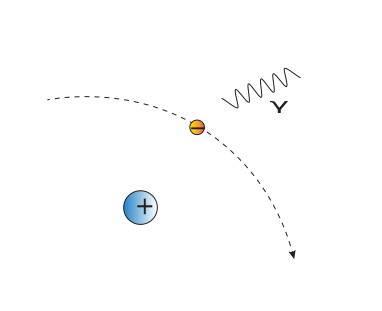
\includegraphics[width=1.0\textwidth]{figures/chapter_3/brem_schematic/brem-schematic-02.png}
\caption{Illustration of Bremsstrahlung process. An electron is scattered by the electric field of a positive nucleus and emits a photon, conserving momentum. }
\end{figure}

Cross sections can be experimentally measured, and also derived from theory. For Bremsstrahlung photons emitted by inelastic scattering from atomic nuclei, the electron cloud of the atom complicates the resulting expressions. Usually the process is complex enough that specific assumptions need to be made for derivations which apply in different energy ranges. For the problem of Bremsstrahlung emission by energetic electrons in the atmosphere, there is a synthesis of theoretical and experimental measurements which can be used to obtain electron energy loss as a function of depth in the atmosphere~ \citep{Berger1972}. Once a Bremsstrahlung photon is produced, it then propagates through the atmosphere and undergoes its own interactions. Photoelectric absorption, multiple scattering, and Compton scattering all have to be taken into account to predict the paths that photons will take in the atmosphere\citep{Berger1972}. This complicates the analysis of the causative electron spectrum significantly. 

Approximations and useful descriptions of the entire process: electron precipitation, the resulting production of X-ray photons, and their subsequent transport through the atmosphere have existed for a long time. An early comprehensive review was carried out by~\citet{Brown1966a}. The first approximations of this processes ignored multiple scattering (\citet{Anderson1960}, \citet{Brown1965}, \citet{Christensen1970}, \citet{Barcus1966}, \citet{KAMIYAMA1966}, \citet{Polk1965}). The first attempt with the effects of multiple scattering included was done by~\citet{Rees1963}. The method used was based on empirical measurements of the energy dissipation of electrons in air.

There are some findings from ~\cite{Rees1963} which can be used to make our analysis of the problem more simple. They note that the effect of the Earth's magnetic field, which can roughly be thought of guiding incident electrons, shouldn't have a significant effect on the energy deposition altitude profiles. This is because above around 70 kilometers, the electron collision frequency greatly exceeds the gyro frequency. Additionally, they argue that since magnetic field lines in the Auroral zone are nearly vertical, changes in electron energy should occur only in the perpendicular direction to the extent that the magnetic field intensity changes in the vertical direction. This should be a small effect, since the strength of Earth's magnetic field does not change appreciably on the relevant vertical scales of kilometers to tens of kilometers. This is a big simplification, because the monte-carlo simulations we will employ are highly sensitive to the simulation spatial scale. Ignoring the effects of the magnetic field allows effects which occur on the scale of the electron gyrofrequency to be ignored, making the simulations much faster. As noted by ~\cite{Berger1972}, the number of photons which survive to detection is small compared to the number of incident electrons. This implies that monte-carlo simulations of the resulting photon spectra will be expensive, so to obtain statistically pure results, simulation speed is important. 

Another important result from ~\cite{Rees1963} is that the initial angular distribution of the precipitating electrons has only a minor effect on the energy deposition profiles, once the total path length through the atmosphere is accounted for. This has two implications: on one hand, the problem of finding X-ray photon spectra corresponding to precipitating electron spectra becomes a single dimensional problem in energy, rather than a two dimensional one in angle and energy. This represents a large simplification. On the other hand, this also implies that obtaining information about the angular distribution of the precipitating electrons from X-ray measurmements is a difficult problem. Our approach in this chapter will be to verify this fact through simulation, and then apply the problems insensitivity to electron angular distribution as a useful simplifying assumption. 

~\cite{Berger1972} provide energy deposition curves for electrons in the atmosphere in a convenient form, providing the number of X-ray photons created per incident electron as a function of electron and X-ray energy, for a given altitude in the atmosphere. These curves are sampled from their data and reproduced in Figures~\ref{berger_seltzer_curves_0}, ~\ref{berger_seltzer_curves_0}, and ~\ref{berger_seltzer_curves_0} for altitudes of 32, 34, and 40 kilometers above ground. The strong dependence on the photon population to the sample altitude is apparent, as well as the characteristic shape of the photon spectra. Their results show that one aspect of the problem that cannot be ignored is the dependence on detector altitude. For a given experiment, this will need to be recorded, and the model run at the same altitude. 

It is prudent to again emphasize at this point that modelling the production of X-rays in the atmosphere caused by precipitating electrons is not a new problem. We need to make a model similar to those of ~\cite{Rees1963} and ~\cite{Berger1972}, not because their results are incorrect, but because we need the flexibility of repeated model runs under different scenarios. Further, when the inverse problem of determining causative electron spectra based on X-ray measurements is attempted in the next chapter, the energy resolution needed in the model output will exceed that of the data provided by these authors.

~\cite{Berger1972} present their results in a useful form, which warrants discussion. Resultant X-ray spectra are presented which correspond to mono-energetic beams of electrons. This can be thought of as a Green's function approach to the modelling problem. Evaluating the model for every input electron spectrum of interest is not necessary, provided that the mapping between the input and output is linear. Since the state of the atmosphere is not altered significantly by incident beams of precipitating electrons in the energy range of interest, different electron beams will produce X-ray spectra which combine additively. For the same reason, the intensity of the resulting X-ray beam will scale linearly with the intensity of the beam of precipitating electrons. In the Green's function approach, beams of mono-energetic electrons are modelled, and the resulting X-ray energy spectra are used to form the columns of a matrix. This matrix then maps between electron energy spectra and X-ray energy spectra for a given altitude. Provided the angular distribution of the incoming electrons can be neglected, and the responses to individual mono-energetic beams can be evaluated to sufficient statistical purity, then model runs for arbitrary precipitating electron spectra can be produced with a single matrix multiplication. 

\begin{figure}[p]
\label{berger_seltzer_curves_0}
\centering
\includegraphics[width=1.0\textwidth]{figures/chapter_3/berger-seltzer-curves/berger_seltzer_curves_0}
\caption{X-ray photon flux per incident electron flux for different incident electron beam energies, from ~\cite{Berger1972}. }
\end{figure}

\begin{figure}[p]
\label{berger_seltzer_curves_1}
\centering
\includegraphics[width=1.0\textwidth]{figures/chapter_3/berger-seltzer-curves/berger_seltzer_curves_1}
\caption{X-ray photon flux per incident electron flux for different incident electron beam energies, from ~\cite{Berger1972}. }
\end{figure}
\begin{figure}[p]
\label{berger_seltzer_curves_2}
\centering
\includegraphics[width=1.0\textwidth]{figures/chapter_3/berger-seltzer-curves/berger_seltzer_curves_3}
\caption{X-ray photon flux per incident electron flux for different incident electron beam energies, from ~\cite{Berger1972}. }
\end{figure}

\section{GEANT4 and Monte-Carlo Simulations}

There are several computer software packages used to simulate the transport of radiation through matter. Two of the most  popular are GEANT4 (GEometry And Tracking), and MCNP (Monte-Carlo N Particle). In this project, we will use the GEANT4 package, since it is open source, and well-documented. The scope of the GEANT4 package is vast, and is used in fields ranging from medical physics to nuclear reactor and detector design. The three main references for the package are~\citet{Agostinelli2003},~\citet{Allison2006}, and~\citet{Allison2016}. GEANT4 is implemented as a set of C++ libraries which provide object-oriented abstractions to nuclear particles and transport processes.  The modularity of this design allows for the creation of simulations with a complexity that can be adjusted to the problem at hand. The simulation we create for predicting X-ray spectra from electron precipitation spectra will use only the necessary components of GEANT4. This is important both for making the resulting program understandable and maintainable, but also for speed. Subjectively, there is no upper limit to the amount of complexity that can be incorporated into this type of software. The aim is to represent only the relevant physics and collect only the data needed for the problem being solved. 

Programs that use the GEANT4 toolkit do so through a defined interface. The structure of a GEANT4 program follows the class diagram shown in Figure~\ref{GEANT4-structure}, which is reproduced from~\citet{Pfeier:519005}. The major components of a GEANT4 simulation are as follows:

\begin{itemize}
\item Detector geometry and readout: The sensitive component of a GEANT4 simulation is called a detector. This is a representation of the physical object in which particle interactions are measured. An example is the sodium iodide crystal in a scintillation detector. The detector is associated with the necessary infrastructure to read measurements, such as, for example, the energy deposition by an incident particle beam.
\item Run / Run Action: An instance of a GEANT4 simulation is called a run. Each run usually consists of a set number of incident particles on the detector.
\item Event: Particle interactions are called events. There are many events for a given run.
\item Tracking: Particles are associated with tracks. Each track is a straight line, which starts and ends with an event. When an event occurs, the simulation physics determine the probability of each interaction along a track.
\item Hits and Processes: A hit represents a specific instance of a particle interaction with the physical materials represented in the simulation. Each hit has parameters such as energy deposition, incident angle, and others associated with it. These quantities can be stored in a histogram when they occur. 
\item Particles and Materials: A particle follows a track in GEANT4 and interacts with the materials represented in the simulation. 
\end{itemize}
 
This is a simplified view of how a GEANT4 simulation works. In reality, simulations created with the toolkit can be arbitrarily complex. A contemporary example would be the simulations used to design the ALICE detector at the Large Hadron Collider. The context in which the major components of the simulation are used can also change depending on the application. For the simulation of electron precipitation, for example, it is sensible to make the representation of the Earths atmosphere the GEANT4 detector. This choice makes it possible to track and record, among other quantities, energy deposition as a function of penetration depth in the atmosphere. The choices made when designing a GEANT4 simulation for a particular experiment need to be done with the understanding that increasing complexity eventually results in diminishing returns. The main focus of this chapter is to develop a simulation which is sufficiently accurate to represent our experiment using a minimal parameter space. 

\begin{figure}[p]
\label{GEANT4-structure}
\hspace{-6cm}
\includegraphics[width=1.7\textwidth]{figures/chapter_3/GEANT4-structure/GEANT4-structure}
\caption{GEANT4 architecture, reproduced from~\citet{Pfeier:519005}. Class structure is in the vertical direction, with dependencies towards the bottom.}
\end{figure}

\section{Representing the Earths Atmosphere}

Precipitating electrons interact with the atoms and molecules which constitute the atmosphere. The simulation needs to account for these constituents. The MSIS-E-90 model~\citep{Picone2002} contains a representation of the main neutral constituents of the atmosphere, as well as their density, and temperature, parameterized by altitude and geographic location. The specific implementation of the model we use in this chapter is written in C++, which makes it compatible with the GEANT4 framework, and is available at \url{https://www.brodo.de/space/nrlmsise/index.html}. This implementation encodes the same data as the original FORTRAN version. Figure~\ref{msis_eval} shows the evaluation of this model as a function of altitude for a specific location on Earth. 

The altitude profiles of Figure~\ref{msis_eval} must be discretized and encoded as a GEANT4 geometry. This is where approximations must be made to keep the model simple enough to be computationally tractable. Each particle interaction in a GEANT4 simulation takes time to calculate and store, but additionally, an ``interaction'' occurs at the end of each particle track. The particle tracks end when a particle reaches a sufficiently low energy, but also when it crosses a physical boundary in the simulation, which exist between the faces of the simulation geometry. It is therefore critical to keep the complexity of the geometry as simple as possible. We choose to define a rectangular, euclidean world, with vertical slices at discrete points representing the atmosphere as a function of altitude. The vertical extent of each slice is chosen to be 1 kilometer, since the major constituents of the atmosphere change density only a small amount on that scale. The horizontal extent of the simulation is set to an arbitrary large number, which for practical purposes can be taken as infinity. This ensures that particle tracks will not terminate by leaving the simulated world through the side boundaries. The model atmosphere is represented to a height of 500 kilometers above ground, beyond which the relevant particle interactions with the atmosphere very rarely occur. 

Each slice of atmosphere in the GEANT4 model is treated as a ``sensitive detector'', which is an abstraction that permits quantities such as energy deposition, entry angle, and the creation of secondary radiation to be recorded as they occur in the simulation. 
    
\begin{figure}[p]
\label{msis_eval}
\includegraphics[width=1.0\textwidth]{figures/chapter_3/msis_eval/msis_eval}
\caption{Evaluation of key MSIS model parameters as a function of altitude. Particularly important for the GEANT4 simulation are the density profiles of each atmospheric constituent (top).}
\end{figure}

A GEANT4 volume is constructed using a stack of three abstractions. First, a G4VSolid is created, representing the shape and dimensions. The G4VSolid can be created from either a small set of geometry primitives (cylinders, boxes, and spheres), or it can be imported from an arbitrary mesh of points. The next component is called a G4LogicalVolume. This abstraction holds a reference to a G4Material, which defines the physical substance that the volume is composed of. The G4Material has the density, temperature, and molecular and atomic components of the volume material specified. The G4LogicalVolume also contains flags which control whether it is a G4SensitiveDetector, or a passive component of the simulation, through which particles are simulated but which does not return data. Finally, a G4PhysicalVolume is created which wraps the rest of the stack into one reference to one object. This object is then placed in the simulation during the initialization routine. 

\section{GEANT4 Physics and Simulation Construction}

Once the physical properties of the GEANT4 are fully specified, a selection of possible interactions between particles is chosen. There are many GEANT4 physics packages available, which are applicable over different energy ranges and for different types of particles. For this project, we will choose the standard electromagnetic physics package~\citep{Burkhardt2004}. This package represents interactions between electrons, photons, and atomic nuclei from energies ranging from MeV down to KeV. Effects that occur primarily below a single KeV, are not represented~\citep{Guatelli2004}. This is a useful approximation for the simulation we construct in this chapter, because it is fast computationally to terminate particle tracks when the reach this energy threshold. Single keV photons and electrons do not travel far in the relevant parts of the atmosphere, and are quickly stopped by the materials surrounding the X-ray instrument. Additionally, the use of a the standard electromagnetic physics package saves development effort and program complexity, since it contains pre-arranged references to all the main interactions we are interested in simulating. 

The input to the atmospheric simulation is specified by electron distributions in incident angle, and energy. Each of these are specified in GEANT4 macro files, which are text files that are used to script GEANT4 applications, and are used to avoid the need to load all the relevant data and inputs at compile time. Topside electron energy and angle distributions can be specified through a list of values, and there are also pre-built functions for the most common forms. For the Green's function approach used for this task, the input energies are a single value which is swept over the relevant energy range (100 KeV to 5 MeV). The question of which angular distribution to use is not obvious, since it depends on the injection process responsible for causing the electron precipitation, the local magnetic field, and possibly other parameters. A Green's function approach here would be complicated, and the resulting simulation would need to span discrete representations of at least two dimensions. It is more practical to fix the angular distribution for a given simulation, and apply a Green's function approach only over the relevant energies. 

It is a general result that only the electron energy spectrum can be retrieved unambiguously from the secondary Bremsstrahlung radiation~\citep{Brown2006}. This indicates that the effect of the angular distribution is small. This is used as the main simplification that we apply in the simulation problem. Choosing a ``reasonable'' angular distribution for the incident electrons and evaluating over only electron energies reduces the simulation a single dimensional problem. This will be critical for the treatment of the inverse problem in the next chapter. 

The inputs to the GEANT4 simulation are then the precipitating electron distribution and total flux. The angular distribution, and the vertical height at which to evaluate the neutral atmosphere model are fixed. The outputs from the GEANT4 simulation are the distributions, in both angle and energy, of the produced X-ray fluxes, along with the total number of X-ray photons in the selected vertical slice of atmosphere. Since the simulation outputs are all integrated quantities, in practice what is done is to select a large arbitrary number for the precipitating electron flux to obtain sufficiently pure statistics in the simulation output, and then to normalize the outputs to this choice. The production of secondary radiation happens less at lower energies, so the chosen incident flux increases towards this limit. Because of this, the most expensive part of the simulation happens when evaluating the effect of low energy (less than 100 KeV) precipitating electrons. Figure~\ref{geant4_io_schematic} shows the inputs and outputs of the GEANT4 simulation schematically. 

\begin{figure}[p]
\label{geant4_io_schematic}
\includegraphics[width=1.0\textwidth]{figures/chapter_3/geant4_io_schematic/geant4_io_schematic}
\caption{Schematic diagram of information flow for a single GEANT4 simulation of energetic electron precipitation and the resulting X-ray radiation}
\end{figure}

The diagram in Figure~\ref{geant4_io_schematic} is the flow of information for a single GEANT4 simulation run. Since we are applying a Green's function approach, this process needs to be repeated across different monoenergetic electron beams. When this is completed, the responses to arbitrary precipitating electron distributions can then be represented as a linear combination of the recorded monoenergetic responses, without requiring further simulation runs for a fixed sample altitude and electron angular distribution. The workflow for applying the resulting data is shown in Figure~\ref{geant4_how_to_use}.

\begin{figure}[p]
\label{geant4_how_to_use}
\includegraphics[width=1.0\textwidth]{figures/chapter_3/geant4_how_to_use/geant4_how_to_use}
\caption{Schematic diagram of information flow for a single GEANT4 simulation of energetic electron precipitation and the resulting X-ray radiation}
\end{figure}

The simulation of all the GEANT4 runs required is computationally expensive. Using the University of Calgary ARC computer cluster, each run was scripted to be run across the required electron energy ranges, and across unidirectional, omnidirectional, and cosine angular distributions. The simulation ranges were then evaluated again over altitudes from 30 to 34 kilometers above ground, which correspond to where viable balloon measurements of the X-ray photons can take place. In total, several weeks of computation across over 100 CPU cores were required. Once this was completed, the results were aggregated and stored in plain text files. While the computation was expensive, the results are compact, and are stored in less than one gigabyte of data. Figure~\ref{geant4-monobeam-results} shows the X-ray results graphically across different altitude ranges.

\section{Validation of Results}

There needs to be a comparison of the GEANT4 simulation results against what already exists in the literature. As stated at the beginning of this chapter, the simulation problem is not new. We are reproducing the work of others so that it may be run over the parameter space we need, especially when attempting to solve the inverse problem. The first published results which we can compare to are by~\citet{Rees1963}. This author presents a semi-empirical form for the results, with a high degree of normalization to the properties of the atmosphere. The work done by~\cite{Berger1972}, on the other hand, is presented in numerical tables in physical units that are close to the output of the GEANT4 simulation. This makes them a good target for comparison to our work. 

The NASA BARREL (Balloon Array for Radiation-belt Relativistic Electron Losses) project has made their modelling work on this problem available through the SPEDAS software package~\citep{Angelopoulos2019}. The BARREL project will be discussed in Chapter~4. For now, we will only use their atmospheric simulation as a comparison to our own work. It is distributed in a format comparable to that used by~\cite{Berger1972}, and can be shown in the same parameter space. Figure~\ref{barrel_berger_spedas_comparison_34} show the expected X-ray flux, in normalized units, for isotropic incident electron beams at varying energies. There is an agreement between the output of our model and the published results. 

\begin{figure}[p]
\label{barrel_berger_spedas_comparison_34}
\includegraphics[width=\textwidth]{figures/chapter_3/barrel_berger_spedas_comparison/barrel_berger_spedas_comparison_alt_40km_3}
\caption{Expected X-ray flux as a function of energy at a sample altitude of 34 kilometers using data from GEATN4 simulations, ~\cite{Berger1972}, and the BARREL SPEDAS model.}
\end{figure}

\section{Problem Separability}

The distributions of photons of a given polar angle and kinetic energy are outputs from the simulation. We will show that the polar angle distribution does not depend on the energy of the precipitating electrons. This allows the results of the simulation to be expressed through their impulse responses in energy only, which is a large simplification. Figure~\ref{photon_angle_independence} shows the polar angle distribution for X-ray photons created by monoenergetic beams of precipitating electrons. Once the total photon counts are normalized to each other, there is no significant difference in the resulting distributions.

We further show that the photon distributions in kinetic energy do not depend on the angular distribution of the precipitating electrons. This important result was originally found by~\citet{Rees1963}, and implies that experiments sensitive to only the energy distribution of bremsstrahlung photons can not recover the angular distribution of the parent electron spectrum. For the attempt at the recovery of the parent energy spectrum in the following chapter, this is useful, since this represents a degenerate dimension of the inverse problem that can be ignored. Figure~\ref{electron_angle_independence} shows GEANT4 simulations of the X-ray energy distributions caused by precipitating beams of electrons following unidirectional (downward), and isotropic angle distributions. 

\begin{figure}[p]
\label{photon_angle_independence}
\includegraphics[width=\textwidth]{figures/chapter_3/photon_angle_independence/photon_angle_independence}
\caption{Polar angle of X-ray photon population at 34 kilometer altitude, as produced by precipitating electrons at different fixed energies. Units are normalized to account for the higher number of photons produced with greater beam energies.}
\end{figure}

\begin{figure}[p]
\label{electron_angle_independence}
\includegraphics[width=\textwidth]{figures/chapter_3/electron_angle_independence/electron_angle_independence}
\caption{Photon energy distribution for 1 MeV incident electron beams having isotropic and unidirectional angular distributions. }
\end{figure}

The final simplification for the simulation problem comes from the parameterization of the detector response. So far we have focused on the creation and validation of the atmospheric model, which gives the angle and energy spectra of the X-ray photons which exist at the detector altitude. The detector output when it is exposed to this population will be a function of this population, and must be modelled through further simulation. The general operating principles and design of the scintillation detectors used in this experiment were described in the previous chapter. For the detector simulation, a GEANT4 model of the geometry is constructed (Figure~\ref{detector_geant4_model}.) 

\begin{figure}[p]
\label{detector_geant4_model}
\includegraphics[width=\textwidth]{figures/chapter_3/detector_geant4_model/detector_geant4_model}
\caption{GEANT4 representation of the detector geometry. The lower plexiglass mount is shown in cyan, the aluminum body in grey, and the led collimator in purple. The height of the complete unit is approximately 30 cm.}
\end{figure}

We examine how the detector geometry selects a population from the X-ray angular distribution. In the detector simulations, an isotropic source of X-ray photons at a fixed energy are created. We run two simulations independently: the first has the entire detector geometry, with its construction materials, enabled. The material corresponding to the sodium iodide crystal, however, is set to a vacuum. This is done to measure the population of photons that reach the crystal, rather than the dynamics of the energy deposition events that happen inside of it. The second simulation is the same, except that the detector materials are set to a vacuum as well as the sodium iodide detector. This provides a baseline which we compare against the first simulation. The distribution of photons which enter the detector geometry will be subset to those recorded when the detector materials are set to a vacuum. Figure~\ref{population_inside_detector} shows the results these two simulations. The lead collimator assembly at the top of the detector has limited the field of view. Some backscatter from the detector materials can also be seen in the first simulation. 

\begin{figure}[p]
\label{population_inside_detector}
\includegraphics[width=\textwidth]{figures/chapter_3/population_inside_detector/population_inside_detector}
\caption{}
\end{figure}

The atmospheric simulation showed that the angle distribution of the X-ray photons does not significantly depend on either the angular distribution of precipitating electrons or their energy distribution. Figure~\ref{population_inside_detector} indicates that the effect of the lead collimator of the detector is essentially to limit the angle from which photons may enter the sodium iodide crystal. Together, this means that the angular portion of the complete problem from electron precipitation, to the creation of x-rays, and finally, to detection, can be largely treated as trivial. To a good approximation, and at the relevant energies (100 keV to 2 MeV), a constant scalar which accounts for the detector field of view can be used to map recorded counts to physical units.

The behaviour of the sodium iodide crystal itself to the absorption of X-ray photons is important and can also be answered through simulation. For this, the detector geometry is fully enabled in the simulation, including the sodium iodide crystal. Rather than the distributions of photon energies and angles within the crystal volume, energy deposition events will be recoded. The energy deposition events correspond to the flashes of light which are amplified by the photomultiplier tube and recorded by the detector electronics. Figure~\ref{detector_energy_response} shows histograms of the energy deposition events for a set of monochromatic photon beams. The responses can be described by delta functions at the corresponding photon energies, with interactions at lower energies which become more complex as the beam energy increases. The main interaction in this energy range is the single deposition of all the photon energy at once, which is why the peaks are easily detectable. 

\begin{figure}[p]
\label{detector_energy_response}
\includegraphics[width=\textwidth]{figures/chapter_3/detector_energy_response/detector_energy_response}
\caption{Energy deposition events inside the detector crystal for beams of monochromatic photons at different set energies. }
\end{figure}



 






%\fancyhead[RO,LE]{\thepage}
%\fancyfoot{}
\chapter{The Inverse Problem}

\section{Geophysical Inverse Problems}

In this chapter the problem of obtaining information about the causative electron precipitation directly from X-ray measurements will be examined. We will term this the ``X-ray inversion problem.'' This type of analysis belongs to the broad class of what are called inverse problems, which attempt to reconstruct physical events based on limited measurement data.  A classic example of such an inverse problem is the determination of media velocities within the Earth based on seismic measurements. The forward problem of predicting instrument responses based on an assumed physical event can be handled by, for example, computer simulations, as was done in the last chapter for the problem of predicting the measured X-ray distributions which result from a given electron precipitation event. As a general rule, inverse problems have certain mathematical properties which make them difficult to solve. We will show the reasons for this, and measures which can be taken to mitigate these effects in this section.

Define the forward problem by the mapping:

\begin{equation}
\mathbf{F}:\mathbf{M} \rightarrow \mathbf{D}
\end{equation}

where $\mathbf{D}$ is the space containing data from measurements, and $\mathbf{M}$ is the space of solutions, which we term models. The mapping $\mathbf{F}$ may be either linear, or non-linear. The inverse problem is:

\begin{equation}
\mathbf{F^{-1}}:\mathbf{D} \rightarrow \mathbf{M}
\end{equation}

 Knowledge of the mapping $\mathbf{F}$ may be incomplete, or based on uncertain experimental data. To describe the challenges associated with inverse problems precisely some definitions are needed.

\theoremstyle{definition}
\newtheorem{definition}{Definition}[section]
\begin{definition}[ill-posedness]
A problem is ill-posed if it fails to have any of the following properties:
\begin{enumerate}
    \item A solution exists.
    \item The solution depends continuously on the input data.
    \item The solution is unique.
\end{enumerate}
\end{definition}

Inverse problems are ill-posed as a general rule. This requires that we shift the analysis from a search for a particular solution, as with forward problems, towards a search for families of solutions, and methods of determining which produce the best description of the available data, often requiring the use of a-priori information about the problem at hand. Based on the results of the last chapter, the X-ray inversion problem certainly satisfies property 1, that a solution exists. The difficulties lie in the failure to satisfy properties 2 and 3. We will show that finding a unique solution to the X-ray inversion problem is, in most realistic cases, not possible. Another definition is needed to see why:

\begin{definition}[ill-conditioning]
A problem is ill conditioned if a small change in the input data results in a large change in the solution, that is, the condition number:

$$\kappa = \lim_{\epsilon \to 0} \sup_{\vert\vert \delta x \vert \vert \leq \epsilon} \frac{\vert\vert \delta f \vert\vert}{\vert\vert \delta x \vert\vert}$$
is large for small changes in the kernel function $\delta f$ and input data $\delta x$.
\end{definition}

 The X-ray inversion problem is ill-conditioned. Figure~\ref{why_ill_conditioned} illustrates this by showing three different model precipitating electron spectra, and a simulation of their resulting X-ray spectra in log-linear space. A small change in the measured X-ray spectrum can result in a drastically different model electron spectrum. The treatment of this instability will be the main problem addressed in this chapter. 

\begin{figure}[p]
\label{why_ill_conditioned}
\centering
\includegraphics[width=1.0\textwidth]{figures/chapter_4/why_ill_conditioned/fig.pdf}
\caption{(top): Example of three different assumed electron energy spectra (mono-energetic, exponentially decreasing, and gaussian) for a precipitating electron flux of $1\times10^9$ electrons per $\mbox{cm}^2$ per second. (bottom): Resulting simulated X-ray spectra for each electron spectrum, using the methods developed in Chapter 3.} 
\end{figure}

\section{Framing the Inverse Problem}

The forward problem of determining instrument responses from electron precipitation events is linear, and can be written as:

$$\mathbf{G}\mathbf{m} = \mathbf{d}$$

where $\mathbf{G}$ is a matrix representing the discretization of the kernel function mapping precipitating electron spectra $\mathbf{m}$ to resulting measurements of the X-ray spectra $\mathbf{d}$. Techniques for computationally determining $\mathbf{G}$ were discussed in the previous chapter. There is a result that allows the calculation of the condition number of $\mathbf{G}$ as the ratio of its maximal and minimal singular values. As a general rule, if a given linear problem has condition number $\kappa$, then we can expect to lose $10^\kappa$ digits of precision in calculating the solution. This is a best-case estimate, since there will also be round-off errors caused by computer floating point representations of the matrix and the data. Techniques to frame the X-ray inversion problem in such a way as to reduce the effect of the ill-conditioning  of $\mathbf{G}$ will be discussed in the this section.

A representation of matrix $\mathbf{G}$ was developed in Chapter~3 using monte-carlo simulations. In that analysis, a Green's function approach is used to write the X-ray spectra resulting from arbitrary input electron spectra as a linear combination of the effects of mono-energetic electron beams. The dimensions of matrix $G$ are determined by the binning scheme used to represent electron and X-ray energy spectra. For the forward problem, the particular binning scheme chosen for both spaces is not critical, provided it is fine enough to capture the scale of the details of interest in both spectra, but coarse enough to support obtaining adequately pure statistics for the resulting X-ray spectra in a practical amount of computing time. For the inverse X-ray problem, however, the binning scheme chosen for kernel function $\mathbf{G}$ has a critical effect on the conditioning of the inverse problem.

To show the effect of choosing different binning schemes for the rows and columns of $\mathbf{G}$, we plot the condition number as a function of bin widths in KeV for the input electron spectra and output X-ray spectra in Figure~\ref{condition_number_binning}. 

\begin{figure}[p]
\label{condition_number_binning}
\centering
\includegraphics[width=1.0\textwidth]{figures/chapter_4/condition_number_binning/fig.pdf}
\caption{Condition number of mapping $\mathbf{G}$ as a function of X-ray spectrum and electron spectrum bin-widths in KeV. The white region is the domain where the condition number is infinite, and $\mathbf{G}$ is singular.}
\end{figure}

Figure~\ref{condition_number_binning} shows that there is a significant set of bin widths which make $\mathbf{G}$ singular. There are also some general trends apparent. Smaller bin widths for the X-ray spectrum tend to reduce the condition number of the problem, as do larger bin widths for the electron spectra. The results from attempting to solve the inverse problem by directly inverting $\mathbf{G}$ are shown for simulated X-ray and electron spectra across different binning schemes in Figure~\ref{direct_inversion_example}.

\begin{figure}[h]
\label{direct_inversion_example}
\centering
\includegraphics[width=1.0\textwidth]{figures/chapter_4/direct_inversion_example/fig.pdf}
\caption{Direct matrix inversion applied to simulated exponential electron spectra with bin widths of 10 (A), 50 (B), and 100 (C) KeV. The incident particle flux is $1\times10^8$ electrons / second / KeV. }
\end{figure}

The direct inversion attempts in Figure~\ref{direct_inversion_example} are an example of a fundamental trade-off encountered when solving inverse problems. Because the information contained in the available measurements is subset to the information contained in the physical event being studied, the best solution, in terms of minimizing residuals between predictions of the resulting model and the data, often has a high variance and contains little useful information. This corresponds to case (A) in Figure~\ref{direct_inversion_example}, where the electron spectrum bin widths are small enough that the model obtained is mostly random noise. On the other hand, choosing wide bin widths as in case (C) can leave relevant information contained in the measurements out of the model, so that while the variance in the solution is low, the model is still not descriptive of the event being studied. This trade-off can be handled through optimization techniques.

\section{Synthetic Data}

The evaluation of techniques to solve inverse problems often depends on the use of synthetically generated, or simulated, data which correspond to solutions which are already known. For the X-ray inversion problem, synthetic data are readily generated using the monte-carlo techniques discussed in Chapter~3. Since the forward problem is linear, X-ray spectra can be generated which correspond to arbitrary electron spectra using a Greens function approach at little computational expense. This represents a power which can be exploited in the analysis of the problem at hand.  

Realistic synthetic data sets always have an error term added, which must be consistent with the statistics of the experiment being simulated. Measuring X-ray spectra is a counting experiment, and therefore the random error associated with the recorded count for a given energy bin has a Poisson distribution. This distribution can be treated as approximately normal for total counts greater than around 10 in each energy bin. This property can be used to simulate an X-ray spectrum which corresponds to an assumed count rate, by adding appropriate noise to the signal produced using the techniques of Chapter~3.

In a real experiment, a measured X-ray spectrum must be background subtracted. The background subtraction is difficult to simulate and is a source of systematic error. Natural sources such as the 511 KeV annihilation line couple with noise inherent to the detector to make a background energy spectrum with a characteristic shape. We will use a sample drawn from experimental data sets to generate a characteristic background spectrum, and then add an appropriately scaled version to synthetic data generated for a given electron distribution and count rate. This approach neglects any systematic error caused by, for example, detector calibration drifting due to temperature changes. 

Due to the sensitivity of the X-ray inversion problem to small perturbations in the measured spectrum, care must be taken when applying tests using synthetic data so as not to introduce a sampling bias in the measured performance of different inversion techniques. It is possible, for example, to combine a particular background subtraction with a simulated spectrum and corresponding measurement noise to obtain a solution to the inverse problem which very nearly matches the assumed causative electron spectrum. This may not be the case when the same test is subsequently run with a different sample of the background spectrum, or a different random seed for the simulated detector noise. For this reason, single tests of an inversion method on one synthetically generated spectrum have no significance. Evaluating a solution technique to the inverse problem on synthetic data is itself an experiment, and must be treated using a sample size large enough to provide significance in the results. 

The data available for this project was obtained using multiple detectors which all had an identical design (discussed in Chapter~3). Since the data set is large, many background samples can be generated for use when creating synthetic data. An example of a ``quiet time'' X-ray spectrum is shown in Figure~\ref{quiet_time_xray}. Over 20 of these background spectra are collected across the available data set, and used to create the average background spectrum shown in Figure~\ref{quiet_time_xray_average}.

Simulated X-ray spectra which are generated using the techniques of Chapter~3 are created without a background component. To account for this in the generation of synthetic data, the average of the available measured background spectra is added to the simulated spectrum, and then a randomly chosen background spectrum is subtracted. We will assume that the differences across all of the measured background spectra can be used as a proxy for the systematic error
expected when a particular background subtraction is applied. 

The complete procedure to conduct a test on an inversion method using synthetic spectra is therefore: 

\begin{enumerate}
    \item An expected X-ray spectrum resulting from an assumed electron distribution is generated using the simulations of Chapter~3. 
    \item Normally distributed noise is added with a standard deviation corresponding to the assumed total X-ray count rate.
    \item The average background spectrum from the available experimental data is added.
    \item A particular background spectrum from the set of experimental data is subtracted.
    \item This process is repeated across the different measured background spectra and across different random seeds for the generated noise, to create a set of synthetic X-ray spectra.
    \item The inversion method being examined is applied across the set of synthetic X-ray spectra, and the resulting inversions are compared statistically with the assumed electron distribution. 
\end{enumerate}

This procedure generates results for one test on a particular inversion method for a particular assumed spectrum. To evaluate the performance of a given inversion method, this entire procedure needs to be repeated across many different assumed causative electron distributions. While the generation of a particular synthetic data set is computationally cheap, the evaluation of the inverse problem can be expensive depending on the technique used. It is, however, absolutely essential that the evaluation of different inversion methods be carried out across a wide data set to avoid sampling bias. This is even more critical when the inversion method being studied is adaptive, depending on the noise level of the input data set. For this case, the entire procedure must be repeated again across different synthetic spectra corresponding to the range of possible count rates.  

There needs to be an objective measure for the relative performance of a given inversion method. The metric should be a scalar, and should increase with the amount of detail that the inversion method captures about the assumed electron spectrum when it is applied to synthetic data. The normalized mean squared error (NMSE) is a simple metric which satisfies these properties. The NMSE is the squared total difference between the retrieved electron spectrum and the assumed electron spectrum, but normalized to the total signal magnitude to account for the fact that it is applied across different count rates. The definition follows.

\begin{definition}[NMSE]
The normalized mean squared error between assumed spectrum $\mathbf{y'}$ and expected spectrum $\mathbf{y}$ is: 

$$\mbox{NMSE}(\mathbf{y},\mathbf{y'}) = \frac{\vert \vert (\mathbf{y} - \mathbf{y'}) \vert \vert}{\vert \vert \mathbf{y} \vert \vert}$$.
\end{definition}

The NMSE is zero for a perfect agreement between a simulated and retrieved electron spectrum, and increases as the agreement becomes worse. Tests on different inversion techniques will produce distributions of the NMSE. These distributions, and particularly their mean and variance, will be the objective measures used for comparing inversion techniques. 

\section{The Least-Squares Regression and the Bias-Variance Trade-off}

Due to the ill-posed nature of the X-ray inversion problem, solutions often take the form of \textit{estimators}. These estimators may be either unbiased, as in the case of least-squares regression, or contain a bias term towards solutions with chosen properties. In Figure~\ref{why_ill_conditioned}, it is apparent that directly solving the X-ray inversion problem using least-squares regression can be ineffective. This is because the problem has a high condition number (Figure~\ref{condition_number_binning}). There is a trade-off apparent for this problem: the condition number can be reduced by selecting coarse binning in model space, which reduces the variance in the solution, but also reduces the amount of information about the data the solution represents. The optimization of this trade-off for a given data set is a basic and well-understood problem in data analysis. A solution is said to be \textit{over-fit} when it aligns well with one data set, but fails to usefully describe the data under small perturbations or additional measurements. On the other hand, a solution is \textit{under-fit} when it fails to reflect significant changes in measurement data. 

Determining the balance between over-fitting and under-fitting a given data set is a basic and well-understood problem in data analysis. Roughly speaking, the variance in the data set is used as a proxy for how much variance is expected in well-fit models which describe the data. The $\chi^2$ statistic is a standard descriptor for this relative variance.

\begin{definition}[$\chi^2$ Statistic]
The $\chi^2$ statistic is the quantity 

$$\chi^2 = \sum_i \frac{(O_i - E_i)^2}{\sigma_i^2}$$

where $\mathbf{O_i}$ are the observed, or measured quantities, $\mathbf{E_i}$ are the expected, or model, quantities, and $\sigma_i^2$ are the variances in the measured quantities. 
\end{definition}

The $\chi^2$ statistic is usually normalized to the number of degrees of freedom which a particular problem has, which gives the reduced $\chi^2$ statistic.

\begin{definition}[Reduced $\chi^2$ Statistic]

The reduced $\chi^2$ statistic is the $\chi^2$ per degree of freedom, $\nu$: $$\chi^{2}_\nu = \frac{\chi^2}{\nu}.$$

\end{definition}

If the reduced $\chi^2$ statistic is much greater than 1, then it indicates a poor model fit. When the  reduced $\chi^2$ statistic is much less than 1, it indicates over-fitting to the data. An example of this is shown in Figure~\ref{overunderfit_example} for polynomial models fit to a randomly generated data set.

\begin{figure}[p]
    \centering
    \includegraphics[width=1.0\textwidth]{figures/chapter_4/overunderfit_example/fig.pdf}
    \caption{Example of over-fit and under-fit models to data. A random data set is generated and polynomial models are fit using least-squares regression. The reduced $\chi^2$ statistic is shown for each model.}
    \label{overunderfit_example}
\end{figure}

Managing the balance over-fitting and under-fitting models is related to the condition number of the problem at hand. If a problem is badly conditioned, as with the X-ray inversion problem, then it may be necessary to under-fit the data to get any useful information from the solution. An example which frequently occurs in test inversions on test data is the existence of negative particle fluxes in predicted electron spectra, an example of which can be seen in Figure~\ref{why_ill_conditioned}. There is no clear way to interpret models with these features. Eliminating them from predicted models is possible using constrained optimization techniques, and will be discussed in the next section. Constrained optimization, combined with other modifications to the least-squares estimator to improve conditioning of the X-ray inversion problem, will be the topic of the remainder of this chapter. 

\section{Biased Estimators and Improving the Condition Number}

The condition number for a given linear problem can be expressed as the ratio of the maximum and minimum singular values in the kernel matrix. Using the singular value decomposition, it is possible to write an alternative version of the X-ray inversion problem with smaller singular values suppressed or removed. The singular value decomposition writes the kernel matrix $\mathbf{G}$ as:

$$\mathbf{G} = \mathbf{U}\Sigma\mathbf{V^T}$$

where $\mathbf{U}$ and $\mathbf{V}$ are unitary, and $\Sigma$ is a diagonal matrix with the singular values on the diagonal. Since the decomposition can be chosen such that the singular values are in descending order, an approximation and reduction in dimensions to the original kernel matrix can be generated by truncating the expansion. Processes like this produce biased estimators, or imperfect representations of data represented by the kernel matrix, in exchange for more solution stability. In this section we will examine the effects of these approximations on the X-ray inversion problem using synthetically generated data from the techniques of Chapter 3. 

Figure~\ref{condition_number_binning} shows that the best binning scheme for the X-ray inversion problem kernel matrix minimizes the bin sizes for the data (X-ray spectra), and maximizes the bin size for the models (electron spectra). This choice must be made within the limits of the statistics of the data set at hand, and the amount of detail desired in the model electron spectrum. As discussed in the previous section, the $\chi^2$ statistic is used to avoid over or under-fitting the problem. Unfortunately, this result is valid only for unbiased estimators, such as the least-squares regression. For a biased estimator, determining the right solution size becomes a much more complicated problem that will be addressed in the next section.

Figure~\ref{singular-value-plots} shows the distribution of singular values across different electron spectrum bin widths. The X-ray spectrum bin widths are left at 1 KeV. Most of the information contained in the kernel matrix is captured in the first few terms of the singular value decomposition. This suggests that reducing the dimensions of the problem by truncating the singular value decomposition might improve its condition.

\begin{figure}[p]
    \centering
    \includegraphics[width=1.0\textwidth]{figures/chapter_4/singular_value_plots/fig.pdf}
    \caption{Plots of the singular values of the kernel matrix for the X-ray inversion problem for different electron spectrum bin widths, with singular values arranged from biggest to smallest.}
    \label{singular-value-plots}
\end{figure}

To justify the use of a biased estimator in solving the X-ray inversion problem, two questions need to be answered. The first is whether or not the use of the biased estimator significantly improves the conditioning of the problem. The second is whether the bias significantly degrades the amount of information contained in the solutions. The first question is easily answered by graphing the condition number of the kernel matrix as a function of truncation index. This is shown as a function of binning scheme in Figure~\ref{condition-number-binning-tsvd}.  

\begin{figure}[p]
    \centering
    \includegraphics[width=.95\textwidth]{figures/chapter_4/condition_number_binning_tsvd/fig.pdf}
    \caption{Plots of the condition number of the kernel matrix for the X-ray inversion problem as a function of electron spectrum and X-ray spectrum bin width, for 1 (A) through 6 (F) truncated singular values.}
    \label{condition-number-binning-tsvd}
\end{figure}

Compared to Figure~\ref{condition_number_binning}, the plots in Figure~\ref{condition-number-binning-tsvd} show that truncating the smallest singular values of the kernel matrix has a positive effect on the conditioning of the X-ray inversion problem. The number of binning schemes which produce a singular kernel matrix, with no inverse, is reduced with increasing truncation index. In addition, the regions with low condition numbers where the inverse problem is tractable (less than $10^3$) are expanded. 

The improved conditioning of the inverse problem by truncating small singular values comes at a significant cost by introducing solution bias. There is no simple method to describe the amount of bias this process introduces, or the effect it will have on a particular data set, however, we can apply the least squares inversion to sample data, as in ~\ref{why_ill_conditioned}, using the truncated kernel and see what effect the bias has. 

Before applying a biased estimator to the inversion problem, there is an important fact which must be made explicit. The main symptom of an ill-conditioned problem is a high sensitivity to small perturbations on the input data. Because of this, one obtains almost no information about the overall behaviour of a given estimator on the X-ray inversion problem by running single tests on synthetic data (which can be generated using the techniques of Chapter 3.) X-ray measurements are counting experiments, and they are subject to statistical noise in their measurements. The statistical noise will follow a Poisson distribution in a well-designed experiment without significant uncorrected detector bias. Since the data have a random component, it would be an error in methodology to attempt to solve the X-ray inversion problem on one specific instance of synthetically generated data. Rather, one should sample a given synthetic data set many times, and then use the inversion technique of choice to see the resulting distribution of computed electron spectra. 

This technique is applied to synthetic electron spectra in Figure~\ref{tsvd_test}. Exponential electron distributions and their resulting X-ray spectra are simulated, and then the X-ray inversion problem is solved using the truncated singular value decomposition and least-squares regression for different truncation indices. The stabilizing effect the truncated SVD approximation has on solutions to the X-ray inversion problem is apparent, though, it is important to note that the spread in the reconstructed spectra due to statistical noise in the simulated X-ray measurements remains significant. In a real experiment, one obtains only one measurement of the X-ray spectrum and the underlying statistical distribution in the noise. This presents a significant problem for reconstructions based on biased estimators, since there is no a-priori way to predict how their characteristic bias will map the noise statistics in measurement space to model space. Despite this problem, and the associated difficulty assigning meaningful error estimates to reconstructed spectra, Figure~\ref{tsvd_test} motivates the search among biased estimators for solutions to the X-ray inversion problem. It is entirely possible, for example, that a measured X-ray spectrum has statistics which only support a binning scheme which makes the inverse problem impossible. A biased estimator, such as truncated singular value decomposition, which effectively improves solution resistance to noise, can be the only way to recover a useful model in these scenarios. 

The use of the truncated singular value decomposition as a biased estimator introduces the truncation index as a free parameter. This leads to an important question: when is the problem well-conditioned enough for the data set being analysed? Higher degrees of truncation improve the conditioning of the X-ray inversion problem (Figure~\ref{singular-value-plots}), but only at the cost of less information being represented in the inverse mapping. The introduction of a free parameter which controls the bias-variance trade-off is a general feature of biased estimators used to solve inverse problems. This too represents a cost, since the choice of this free parameter must be somehow justified. The question then becomes whether there is a method to choose this parameter based on data from a given experiment. This question is central to the X-ray inversion problem, and is the focus of the remainder of this chapter. 

\begin{figure}[p]
    \centering
    \includegraphics[width=.95\textwidth]{figures/chapter_4/tsvd_test/fig.pdf}
    \caption{Plots of simulated electron spectra for a total electron flux of $1\times10^9 \mbox{electrons} / \mbox{cm}^2 / \mbox{second}$, and their reconstruction from the associated simulated X-ray spectra using a truncated singular value approximation of the kernel matrix. Electron bin widths are set to 50 KeV, and X-ray bin widths to 1 KeV. (A), (B), and (C) show reconstructions with the smallest 1, 5, and 10 singular values dropped from the expansion.}
    \label{tsvd_test}
\end{figure}

\section{Tikhonov Regularization and the L-Curve Method}

The truncated singular value decomposition explored in the last section is not the only method which has been developed to recondition inverse problems. For the optimization problems that arise from the introduction of a free parameter with biased estimators, it is desirable to have a continuous variable which controls the degree of reconditioning, rather than a discrete truncation index. Further, it is useful to have an estimator which exhibits a bias towards certain families of solutions, using a-priori knowledge we might have about the shape of the expected solution to the inverse problem. The method of Tikhonov regularization has these properties.

In Tikhonov regularization, the unbiased least-squares regression:

$$\min_{\mathbf{x}} \vert \vert \mathbf{A} \mathbf{x} - \mathbf{b} \vert \vert $$

is replaced with the modified version:

$$\min_{\mathbf{x}} \vert \vert \mathbf{A} \mathbf{x} - \mathbf{b} \vert \vert + \alpha \vert \vert \mathbf{x} \vert \vert.$$

The parameter $\alpha$ is a positive real number which controls the strength of the regularization. When $\alpha$ is zero, the least-squares solution is recovered. The addition of $\alpha \vert \vert \mathbf{x} \vert \vert$ to the least-squares minimization represents a penalty term on the size of the solution norm. There is a close relationship between the effect of adding this penalty term and the suppression of small singular values in the kernel matrix. Write the singular value decomposition of the kernel matrix as:

$$\mathbf{G} = \mathbf{U}\Sigma\mathbf{V^T}.$$

It can be shown that the solution to the Tikhonov regularization can be written as:

$$\mathbf{x} = \mathbf{V}\mathbf{D}\mathbf{U}^T \mathbf{b} $$

where the diagonal values of $\mathbf{D}$ are:

$$\mathbf{D_{ii}} = \frac{\sigma_i}{\sigma_i^2 + \alpha^2}$$

where $\sigma_i$ are the singular values of $\mathbf{G}$. The regularization term applies a filtering effect which smoothly suppresses the smallest singular values in the kernel matrix. This effect improves the condition number of the kernel matrix, and stabilizes solutions to the inverse problem. This is accomplished at the cost of a bias towards solutions with a small norm, which scales with the degree of regularization applied. 

Tikhonov regularization has a heuristic interpretation. The deviation from a solution with a small norm can be viewed as a measure of its complexity, and the amount of information which it contains. The trade-off between solutions to inverse problems with stability but high bias, and solutions with small residual errors but high variance, is controlled by the regularization parameter $\alpha$. There is no single method to choose an appropriate value for $\alpha$ for a given problem. Techniques to select $\alpha$ can include heuristic arguments, a-priori knowledge based on the properties of the particular problem at hand, and statistical arguments. Combinations of these methods are also possible, but all of them represent an implicit cost to the analysis of the problem at hand, namely, that a choice in $\alpha$ ultimately needs to be made, and that choice will always depend, to an extent, on the preferences of the analyst. This is a danger to the analysis of the X-ray inversion problem, which we will mitigate through careful testing on synthetic data across multiple techniques, and objective scoring of different techniques using clearly defined metrics. 

The classic method for choosing $\mathbf{\alpha}$ is the so-called ``L-curve''. This heuristic method works by plotting the solution norm $\vert\vert \mathbf{x} \vert\vert$ vs the error term $\vert \vert \mathbf{A}\mathbf{x} - \mathbf{b} \vert \vert$ in log-log space. Typically, but not always, this plot has a characteristic L shape, with an inflection point which locates the value for $\alpha$ that produces the most significant reduction in solution norm for the smallest error term. If the error term is thought of as the cost of solution stability, then the inflection point locates the most economical value of $\alpha$. 

An example of this applied to the X-ray inversion problem is shown in Figure~\ref{l-curve-example}. We use a synthetic X-ray spectrum based on an exponential beam of electrons with a folding energy of 300 KeV. The L-curve is shown and used to select $\alpha = 2.0\times10^{-5}$. The assumed electron spectrum is plotted along with spectra determined using direct matrix inversion, and Tikhonov regularization for the selected value of $\alpha$. Multiple runs across synthetic data generated with different random seeds are used to provide an accurate representation of the variance in each solution. 

\begin{figure}[h]
    \centering
    \includegraphics[width=1.1\textwidth]{figures/chapter_4/l-curve-example/fig.pdf}
    \caption{Application of Tikhonov regularization and the ``L-curve'' method to synthetic exponential electron spectrum. The assumed electron spectrum is shown in blue (bottom, left), and the retrieved spectra are shown for direct inversion (grey) and Tikhonov regularization (green).  }
    \label{l-curve-example}
\end{figure}

The reduction in variance gained from the regularization process is evident in Figure~\ref{l-curve-example}. The spread in solutions using direct inversion is large enough, that besides a general trend towards a decrease with lower energies, few other features are readily apparent. Additionally, some of the direct solutions show negative particle fluxes in the lower energy bins. Without careful analysis of the variation in solutions caused by the counting statistics, inversions attempted using experimental data could even be misleading, showing apparently significant features which are in fact only caused by the mapping of random noise through the ill-conditioned kernel matrix of the problem. 

The bias introduced by regularization is also apparent in Figure~\ref{l-curve-example}. Towards lower energies the solution trends downward, which is a feature the assumed electron spectrum does not have. The spectrum retrieved using regularization is also not fully exponential, and a folding energy retrieved by fitting an exponential curve would have a non-zero error when compared with the assumed data. Although the variance in the direct solution is large enough to be untenable when applied to experimental data, it remains exponential, and on average, the folding energy will match the assumed model. 

Unfortunately, there is no general method to assign useful confidence intervals to solutions from biased estimators, including those generated from Tikhonov regularization. The effect of the variance in solutions is simple enough to capture, as done in Figure~\ref{l-curve-example} by running the inversion multiple times under different random seeds, but a true confidence interval would include the effects of both the bias and the variance in the solution. The use of a biased estimator such as Tikhonov regularization  makes an otherwise unsolvable problem tractable, but only at the cost of the certainty and bounds we can place on the solutions. In a way, an ill-posed problem represents a mismatch between the amount of information contained in the solution, and the amount of information in the available data. Tikhonov regularization allows us to control the manifestation of this fundamental lack of information, but there is no process by which it can be eliminated. 

For all the caveats and drawbacks which come with applying Tikhonov regularization to a problem, it has a critical property which the unbiased methods lack - namely that it is \textit{adaptive}. The method works by balancing the variance in the solution against the norm, which means that as data become noisy and harder to resolve, the bias is increased to compensate and maintain stability. This is in sharp contrast to, for example, choosing a binning scheme or parameterization which remains fixed for a given problem. Some data sets are ``easier'' to invert through a given kernel matrix than others, which can be for a multitude of reasons. For example, the data set could represent a monochromatic solution, which incurs the least variance-inducing resistance in the inversions. Tikhonov regularization is sensitive to this fact, and the L-curve will have a shape which corresponds to the particular problem and particular data set at hand. 

The L-curve method is computationally expensive, since solutions need to be generated for every value of $\alpha$ being examined. For relatively small matrices, say, less than 1000 by 1000 rows and columns, this is a small problem, but it becomes significant as the problem being examined scales. Because of this, when using Tikhonov regularization, the most sensible binning scheme for the X-ray inversion problem is not necessarily the one which provides the finest resolution in X-ray spectra, as Figure~\ref{condition_number_binning} would suggest. Practical considerations based on computational limits need to be taken into account. 

The fact that the L-curve method is somewhat heuristic motivates us to look for another way to select a value for $\alpha$. The ``corner'' of the L-curve plot, if it appears, is not always sharp. This represents a way that the expectations of the human doing the analysis can find their way into the solutions created using Tikhonov regularization. There is a family of related methods which can be used to select $\alpha$ based on the statistical properties of the data alone. The cross-validation methods use the idea that the artificial removal of parts of the input data produce different solutions and can give information about the stability of the problem being analysed. In particular, under the hypothesis that the effect of the removal of a single data point, such as a single energy bin in the X-ray inversion problem, should have only a small effect on the retrieved electron spectrum. Iterating over the available energy bins, and suppressing each one from the problem in turn, will produce a spread of solutions, whose variation gives a picture of the overall stability of the inversion. If this entire process is repeated over different values of $\alpha$, then the total mean squared error between the suppressed data points and the regularized solutions is can be compared and minimized. This process is motivated schematically in Figure~\ref{cross_validation_motivation}. In both the over-fit and under-fit cases, the missing data point is fit poorly. Minimizing this effect represents a balance between these cases and produces a corresponding value for $\alpha$. 

\begin{figure}[p]
    \centering
    \includegraphics[width=1.0\textwidth]{figures/chapter_4/cross_validation_motivation/fig.pdf}
    \caption{Random data set (blue) with under-fit (orange), and over-fit (green) representations. A particular data point (red) is removed prior to fitting. The removed data point is far from both the over-fit and under-fit representations of the data. }
    \label{cross_validation_motivation}
\end{figure}

Iteration over one suppressed data point is called leave one out cross-validation. It is also possible to leave out any number of data points up to $n-1$, where $n$ is the total number of points in the data set. For leave n out cross validation, one evaluates the solutions generated by every possible way to suppress n data points. This is incredibly computationally expensive. 

In Figure~\ref{cross-validation-example}, the synthetic data set from Figure~\ref{l-curve-example} is reproduced, but $\alpha$ is selected using leave-one-out cross validation. Minimizing the mean-squared error using the cross-validation method suggests $\alpha=7.8\times10^-2.$ This is a different value from what was used in Figure~\ref{cross-validation-example}, but the retrieved spectrum is approximately the same. This suggests a degree of stability across values of $\alpha$ for the application of Tikhonov regularization to the X-ray inversion problem, but testing across many data sets is required for verification. This will be attempted towards the end of this chapter, where the different regularization methods are compared across a large set of synthetic data sets. 

Unlike the ``L-curve'' method, cross-validation leaves no room for the human analysing the problem to have input on the regularization parameter $\alpha$. Instead of looking for an inflection point on a log-log graph, which has some room for interpretation, the minimization of squared errors across values of $\alpha$ for cross-validation is carried out numerically. The minimum located in Figure~\ref{cross-validation-example}, for example, is quite sharply defined. This lack of interpretation is a strength of the cross-validation method. Further, since the minimization process requires no human intervention, it can be  applied to large bodies of synthetic data automatically. This is useful both for running on synthetic data for testing, as well as different sets of experimental data. Since the objective characterization of the performance of an inversion technique to the X-ray inversion problem will depend on its application across to synthetic data, this strength is important. 

\begin{figure}[p]
    \centering
    \includegraphics[width=1.1\textwidth]{figures/chapter_4/cross-validation-example/fig.pdf}
    \caption{Application of Tikhonov regularization and the leave-one-out cross-validation method to synthetic exponential electron spectrum. The assumed electron spectrum is shown in blue (bottom, left), and the retrieved spectra are shown for direct inversion (grey) and Tikhonov regularization (green).}
    \label{cross-validation-data}
\end{figure}
\newpage
\section{Higher Order Regularization}

The process of Tikhonov regularization can be interpreted as the addition of a-priori information to the problem. In Tikhonov regularization, the modified least-squares problem:

$$\min_{\mathbf{x}} \vert \vert \mathbf{A} \mathbf{x} - \mathbf{b} \vert \vert + \alpha \vert \vert \mathbf{x} \vert \vert$$

has a penalty term  $\vert \vert \alpha \vert \vert \mathbf{x} \vert \vert$ introduces a preference for solutions with a smaller norm. This was motivated by the fact that more complex solutions typically have a larger number of non-zero terms than simpler solutions, and, to introduce stability, the strength of the regularization should increase with solution complexity. This was indicated graphically through the L-curve method. There are other forms for the penalty term, which can be chosen to align with the properties of physically reasonable solutions to the problem at hand. This section will examine these higher-order regularization terms as applied to the X-ray inversion problem. 

Write a new least-squares problem as:

$$\min_{\mathbf{x}} \vert \vert \mathbf{A} \mathbf{x} - \mathbf{b} \vert \vert + \alpha \vert \vert \mathbf{L} \mathbf{x} \vert \vert$$

where $\mathbf{L}$ is a linear operator. If $\mathbf{L}$ is the identity matrix, then the ordinary regularization is recovered. This is termed zeroth-order tikhonov regularization. In first-order tikhonov regularization, $\mathbf{L}$ is chosen to be the matrix which approximates the first derivative operator:

\[
\mathbf{L} = \begin{bmatrix} 
    1 & -1 & 0 & \dots \\
    0 & 1 & -1 &\dots \\
    \vdots & \ddots & \\
    0 & \dots & 1 & -1 
    \end{bmatrix}
\].

Unlike zeroth-order regularization, which prefers small solutions, this choice of $\mathbf{L}$ penalizes solutions which change - the preference is for constant solutions. For problems where we have an a-priori expectation that solutions are constant, this operator would be the clear choice. A useful and interesting feature of first-order regularization is that no advance knowledge of the best constant solution needs to be applied. 

For the X-ray inversion problem, we do not have any strong expectation that solutions will be constant. In fact, it is more reasonable that electron fluxes decrease as a function of energy. This is motivated by both satellite observations, and balloon flights where models of exponentially decreasing electron spectra tend to best describe measured X-ray data. This motivates the search for a different penalty term for the regularization problem, which better matches this expectation. 

Second-order Tikhonov regularization uses a linear operator which approximates the second derivative:

\[
\mathbf{L} = \begin{bmatrix} 
    1 & -2 & 1 & 0 & \dots \\
    0 & 1 & -2 & 1 & \dots \\
    \vdots & \ddots & \\
    0 & \dots & 1 & -2 & 1 
    \end{bmatrix}
\].

This operator introduces a preference for smooth solutions. There is an intuitive reason why using this operator for the X-ray inversion problem might be useful - as the noise in the measured X-ray spectrum increases, the number of features detectable in the model electron spectrum will go down. A relevant example would be an electron spectrum which is well-described by two beams at different energies. For low noise levels in the corresponding measured X-ray spectrum, the two beams can be resolved through direct inversion, without applying regularization. As the noise in the measured spectrum is increased, second-order regularization will dull and blend the two sharp peaks until eventually they are not distinguishable.  This is a desirable property, since the bias tends towards solutions which reflect the lack of information a high noise measurement represents. This is illustrated in Figure~\ref{two_peak_second_order_example}.

\begin{figure}[p]
    \centering
    \includegraphics[width=1.1\textwidth]{figures/chapter_4/two_peak_second_order_example/fig.pdf}
    \caption{Application of second-order Tikhonov regularization to synthetic X-ray measurements corresponding to two mono-energetic electron beams at different X-ray fluxes and noise levels (A - $10^7$ electrons / sec / keV, B - $10^6$ electrons / sec / keV, C - $5\times10^5$ electrons / sec / keV)}
    \label{two_peak_second_order_example}
\end{figure}
\newpage

An additional argument for applying second-order Tikhonov regularization to the X-ray inversion problem is that completely sharp, mono-energetic features aren't realistic in natural electron spectra. Thermal processes tend to relax such distributions to have a characteristic width, and over a long enough time period, the central limit theorem tends them towards Gaussian distributions regardless. Since sharp solutions aren't generally expected, it makes sense to choose $\mathbf{L}$ such that they are penalized. This represents further injection of a-priori information to the problem.  

\section{Constraints and Preconditioning}

The application of regularization techniques makes the X-ray inversion problem tractable, with realistic and imperfectly measured input data. In using a biased estimator, we have replaced an impossible linear problem with a condition number approaching $10^{10}$, with a nearby problem that is better behaved. The cost of this is an artificial tendency towards families of solutions influenced by a-priori information, such as smooth solutions, for second-order Tikhonov regularization. The effect of this bias increases with noise in the input data. In this section, we explore methods which can be used to apply simplifying transformations to the X-ray inversion problem prior to the regularization process. Provided that the transformations applied have an inverse, they can be used to re-cast the X-ray inversion problem as an equivalent linear problem in a different space. If the transformations applied are chosen carefully, the equivalent problem can have a condition number which is significantly reduced. This reduces the amount of regularization that needs to be applied for stability, or equivalently, allows more information to be obtained from noisy measurement data. 

As a motivating example, take the linear problem $\mathbf{A}\mathbf{x} = \mathbf{b}$, with $\mathbf{A}$ defined as:

\[
\mathbf{A} = \begin{bmatrix} 
    .0001 & 1.0001 & 0 \\
    0 & 1 & 0 \\
    0 & 0 & 1
    \end{bmatrix}
\].

The condition number of $\mathbf{A}$ is approximately $2.0\times10^{4}$. Instead of calculating $\mathbf{A}^{-1}$, first left and right multiply by linear transformation:

\[
\mathbf{L} = \begin{bmatrix} 
    100 & 0 & 0  \\
    0 & 1  & 0 \\
    0 & 0 & 0
    \end{bmatrix}
\].

The new matrix is:

\[
\mathbf{\tilde{A}} = \begin{bmatrix} 
    1 & 100.01 & 0  \\
    0 & 1  & 0 \\
    0 & 0 & 1
    \end{bmatrix}
\].

with a condition number of $1.0\times10^{4}$. The corresponding transformation can be applied to $\mathbf{b}$ to obtain the solution, $\mathbf{x}$, of the original problem. This preconditioning can be applied before using regularization methods, reducing the amount of regularization required for stability with a  particular problem and data set. 

In general the left and right-multiplication can be done using different matrices. Label the left preconditioner $\mathbf{L}$ and the right preconditioner $\mathbf{R}$. The linear problem:

$$\mathbf{A}\mathbf{x} = \mathbf{b}$$

can then be recast as:

$$(\mathbf{L}\mathbf{A}\mathbf{R}^{-1}\mathbf{R})\mathbf{x} = \mathbf{L}\mathbf{b}.$$

Since the X-ray inversion problem is linear, there is no inherent cost to applying preconditioning methods before solutions are found. Provided matrices $\mathbf{L}$ and $\mathbf{R}$ are not singular, the solution to the original problem can be recovered. 

There is no known general method to determine optimal values for $\mathbf{L}$ and $\mathbf{R}$. There are some specific cases, such as for symmetric matrices, where techniques exist, but the matrix which describes the X-ray inversion problem does not fall into any of these categories. This problem makes finding an appropriate preconditioner for the X-ray inversion problem non-trivial. We will try different combinations of known preconditioners, and stop when a selection is found that significantly reduces the condition number of the problem. 

From a computational perspective, the ``ideal'' matrix representing the X-ray inversion problem would be the identity, with a condition number of one. Compared to the identity matrix, the real matrix representing the X-ray inversion problem has two main undesirable properties. The first is that the rows, which represent X-ray spectra from mono-energetic beams of electrons, have a high degree of col-linearity. This is the main cause of the high condition number of the matrix. The second problem is that the rows and columns have vastly different norms. This is because low energy beams of electrons do not penetrate far into the atmosphere, and their impact in terms of measurable X-rays is small. On the other hand, high energy beams of electrons need only have a small total particle flux to create a very large measurable X-ray response. Figure~\ref{matrix_spectral_plot} (top) shows this for a particular binning scheme on the response matrix though graphs of its rows. The spectrum of singular values is also shown. We will show that preconditioning can have a significant effect on the singular values of the resulting matrix. 

\begin{figure}[p]
    \centering
    \includegraphics[width=1.1\textwidth]{figures/chapter_4/matrix_spectral_plot/fig.pdf}
    \caption{(left): Graph of the rows of the X-ray response matrix. A high degree of co-linearity is apparent, as with a large scale change between rows. (right): Graph of the singular values of the X-ray response matrix, from largest to smallest. }
    \label{matrix_spectral_plot}
\end{figure}

One classic left-preconditioner is called diagonal scaling. For this preconditioner, a diagonal matrix is constructed such that the entries are equal to the inverse of the norm of the rows of the target matrix. This has the effect of making the row norms of the transformed matrix closer together. Figure~\ref{matrix_spectral_plot} (bottom) shows the effect of applying this preconditioner. The row norms and the spectra of singular values span fewer orders of magnitude. For this example, diagonal scaling has improved the response condition number from a value of $1.6\times10^4$ to $1.3\times10^4$. This is not a big change, at least not large enough to see a significant difference in the degree of regularization required to stabilize the X-ray inversion problem, but it is a reduction, and it motivates a search for other, perhaps more effective, preconditioners to use. 

The effect of the diagonal scaling preconditoner can also be seen across different binning schemes on the X-ray response matrix. The effect is not constant across binning schemes. This is shown in Figure~\ref{matrix_spectral_plot_diagonal_scaling}.

\begin{figure}[p]
    \centering
    \includegraphics[width=.8\textwidth]{figures/chapter_4/condition_number_binning_diagonal_scaling/fig.pdf}
    \caption{(top): Contour plot of the condition number of the X-ray response matrix as a function of electron spectrum and X-ray spectrum bin widths, with no preconditioner. (bottom): The same contour plot with diagonal scaling preconditioner applied.}
    \label{matrix_spectral_plot_diagonal_scaling}
\end{figure}

Calculating the condition number of a matrix requires computing the singular value decomposition, which is a well known and optimized process and can be done very quickly on modern computers. As an experiment, we can think of the condition number as a function of the diagonal entries of the preconditioning matrix and attempt to minimize it, using, for example, a conjugate gradient search. Despite the fact that this represents a problem with many dimensions, this simple idea can produce a right preconditioner which is effective. An example of the application of this process is shown in Figure~\ref{optimized_left_preconditioner}.

\begin{figure}[p]
    \centering
    \includegraphics[width=1.1\textwidth]{figures/chapter_4/optimization_left_preconditioner/fig.pdf}
    \caption{(top left): Rows of the response matrix with an optimized diagonal preconditioner applied. (top right): corresponding spectra of singular values for the response matrix. (bottom): condition number as a function of iteration number for a conjugate gradient optimization of the preconditioner matrix entries}
    \label{optimized_left_preconditioner}
\end{figure}

It is clear that there are different matrices that can be selected to improve the condition of the X-ray inversion problem. Since one can generally expect to lose $k$ digits of precision for a linear problem with a condition number of $10^k$, the search for an optimal preconditioner for the problem at hand isn't very sensitive. Significant benefits will only be returned if order of magnitude improvements in the condition number can be found. This can be achieved through regularization, but comes at the cost of a bias which is difficult to quantify. Because of this, the best approach to the X-ray inversion problem is a combination of left and right preconditioners, chosen optimally for a given selected binning scheme, combined with a regularization method. This dual approach obtains the full benefit of any preconditioners, with the stability, at a cost, which regularization provides. Since the regularization techniques are adaptive to both the noise in the measurement data and the inherent conditioning of the problem, the result is that regularization is used ``as little as possible'', to obtain stability in the solution. 

Choosing left and right preconditioning through optimization techniques generally works to reduce the condition number of the problem, but there are opportunities for it to fail, such as the numerical optimizer failing to converge. Additionally, there is a risk that the optimization adjusts preconditioning based on noise in the response matrix, which is generated through simulations, rather than the inherent shape of the response curves the matrix contains. This can be seen to an extent in the lower energy limit in Figure~\ref{optimized_left_preconditioner}. The danger with this effect is that the collinearity of the component vectors of the response matrix is reduced only for synthetic data generated with the same response matrix. Real experimental data will not benefit from this reduced collinearity, since their noise statistics are independent of the response matrix. 

An intuitive and useful pair of left and right preconditioners for the X-ray inversion problem can be created based on the observation that the response matrix is poorly scaled in both rows and columns. This is illustrated in Figure~\ref{matrix_scaling_plot}, which shows that the row and column norms differ through orders of magnitude across the response matrix.

\begin{figure}[p]
    \centering
    \hspace*{-2.5cm}
    \includegraphics[width=1.1\textwidth]{figures/chapter_4/matrix_scaling_plot/fig.pdf}
    \caption{Response matrix for the X-ray inversion problem.  }
    \label{matrix_scaling_plot}
\end{figure}
\chapter{Experiment Data and Analysis}

\section{Overview of The Balloon Experiments}

High altitude balloons have an extensive heritage as platforms for experiments that take place in the upper atmosphere. In this chapter we will examine results from three balloon flight campaigns which carried X-ray spectrometers. The results of the previous chapters will be applied to determine as much information about the causative precipitating electrons as possible, while avoiding over-fitting the available data. The total precipitating flux and energy distribution of the electrons will be the main targets. The experiments on the balloon flights that we use in this chapter were all equipped with NaI scintillator detectors, and the analysis will be framed around the data that can be obtained from them. There will be questions that can be answered using detectors of a different design, particularly, those sensitive to the angular distribution of the incoming photons. These will be discussed at the end and left for future work. 

The balloon flights used in this analysis were from the following campaigns.

\begin{center}
\begin{tabular}{ |c|c|c|c| } 
\hline
Project Name & Location & Active & Primary Reference \\
\hline
$\text{ABOVE}^2$ & Saskatoon, Saskatchewan & Summer 2016 & None Current\\
\hline
BARREL & Antarctica & 2013-2014 & \citet{Millan2014}\\
\hline
EPEX & Fort MacMurray, Alberta & Summer 2018 & None Current\\
\hline
\end{tabular}
\end{center}

The campaigns each consisted of a number of flights. Each had a somewhat different scientific target, which will be discussed in their analysis sections, however, all of them carried NaI scintillation detectors of a similar design, which we can use with the results from the previous two chapters. We will begin with a discussion of the detector design and operating principles. 

\section{Detector Design}

The sodium iodide scintillation detector carried by flights on all three balloon campaigns was designed by Dr. Michael McCarthy at the University of Washington, Seattle campus. The instrument design has a heritage extending back to~\citet{winckler}. The instrument specifications for the BARREL campaign flights follow, reproduced from~\citet{Millan2014}. 

\begin{center}
\begin{tabular}{ |c|c|c|c|c| }
\hline
Attribute & Value & Comments \\
\hline
Mass & 2.8 Kg & includes insulation and harness \\
Energy Range & 20 keV to 10 MeV & \\
Electronics Resolution & 2.4 keV / channel & reduced by binning \\
System Resolution & 7 percent at 662 keV & \\
Effective Area & 16$\text{ cm}^2$ at 1 MeV & \\
Dead time Per Event & 52 $\mu\text{s}$ & \\
Operating Temperature & -10 to 40 deg C & efficiency decreases below 15 deg C \\
Voltage Requirement & +/- 5 V DC & \\
Current Requirement & 40 mA +, 10 mA - & depends on count rate\\
\hline
\end{tabular}
\end{center}

Simulations completed with GEANT3 (the predecessor to GEANT4) indicate that the detector behaves as essentially uncollimated, though the view through the atmosphere results in it having a field of view of approximately 60 degrees~\citet{Millan2014}. 

A picture of the detector as flown on the $\text{ABOVE}^2$ campaign is shown in Figure~\ref{detector_picture}. The unit is cylindrical, standing on a plexiglass mount and standing approximately 30 cm tall. The cylinder includes the NaI scintillation crystal, photomultiplier tube, and optical coupling. X-rays deposit their energy in the NaI crystal, and a fraction of the resulting light pulse is converted to a voltage pulse by the photomultiplier tube~\citet{Millan2014}. This voltage pulse is then converted to a digital value proportional to the deposited energy by the DPU and output on a serial port for processing and storage by the rest of the flight system. The disconnected wire harnesses visible in Figure~\ref{detector_picture} connect the detector to the various support hardware included with the flight system. Temperature sensors and heaters were used to maintain the detector temperature at 15 deg. C during the flight. Power was provided by an array of lithium-ion rechargeable batteries, which are contained in the rectangular foam box behind the detector in Figure~\ref{detector_picture}.

\begin{figure}[p]
    \centering
    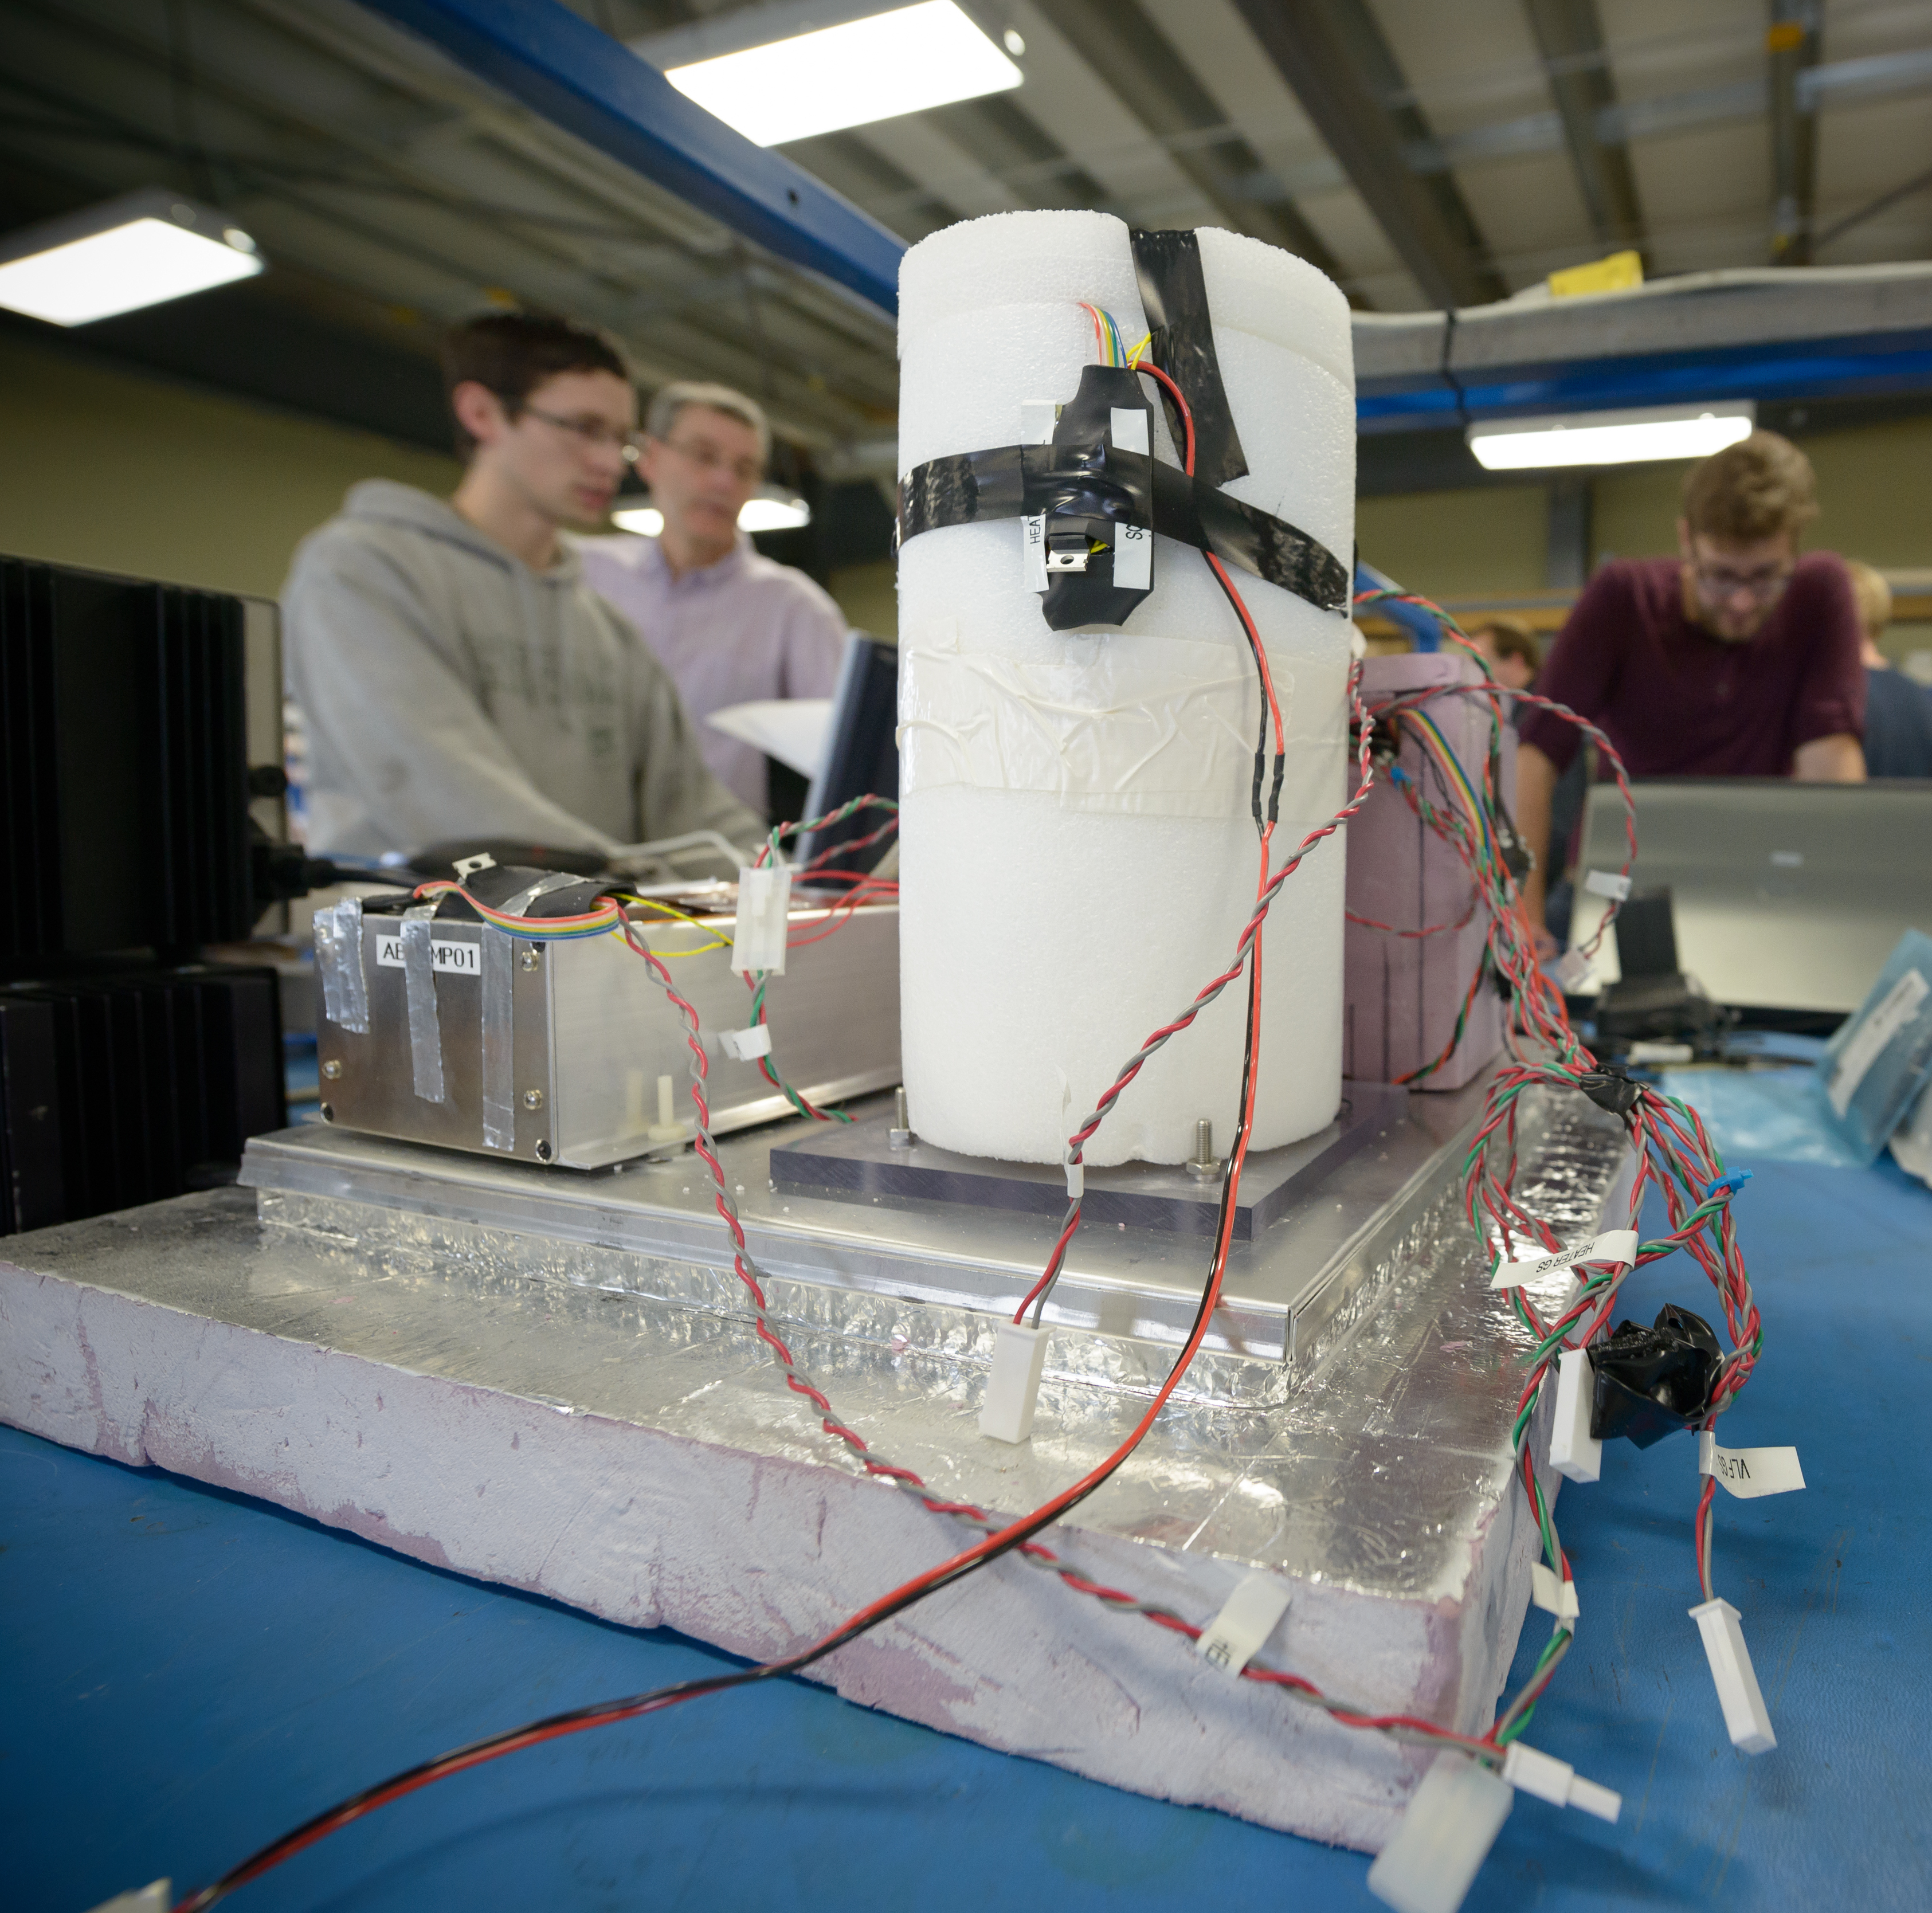
\includegraphics[width=1.0\textwidth]{figures/chapter_5/detector_picture/detector_picture.jpg}
    \caption{X-ray spectrometer (white cylinder) encased in insulation foam and installed with flight systems in balloon payload. The DPU (digital processing unit) is contained in the metal rectangular enclosure on the left. The lead collimator assembly is hidden under the white styrofoam insulation.}
    \label{detector_picture}
\end{figure}

The detector sends measurements to a serial port as digital data. The outputs, reproduced from~\citet{Millan2014}, follow.

\begin{center}
\begin{tabular}{ |c|c|c|c|c| }
\hline
Product & Cadence & Energy Range (keV) & No. of Energy Channels \\
\hline
Rate Counters & 4 & - & - \\
Fast Spectra & 0.05 & 20-1500 & 4 \\
Medium Spectra & 4 & 100-4000 & 48 \\
Slow Spectra & 32 & 20-10000 & 256 \\
\hline
\end{tabular}
\end{center}

For the EPEX and $\text{ABOVE}^2$ campaigns, the instruments were designed to be recovered, and the data were recorded to onboard storage, with some telemetered results as a backup. For the BARREL campaign, the logistics involved in recovering all the payloads are difficult. While a subset were recovered, most were not, and the data were telemetered using an iridium satellite modem. For these flights, the analysis uses the data products published at NASA CDAWEB. The primary citation for this data set is~\citet{Millan2014}.

The functional layout of the detector is shown in the block diagram of Figure~\ref{detector_block_diagram}, which is reproduced from~\citet{Millan2014}.

\begin{figure}[p]
    \centering
    \includegraphics[width=1.0\textwidth]{figures/chapter_5/detector_block_diagram/detector_block_diagram}
    \caption{Block diagram of X-ray scintillation detector system}
    \label{detector_block_diagram}
\end{figure}

\newpage

\section{The $\text{ABOVE}^2$ Campaign}


The $\text{ABOVE}^2$ balloon campaign was flown during the Summer of 2016. There were three flights, each using zero-pressure balloons manufactured by Near-Space Corporation, and designed for a float altitude of greater than 33 kilometers. The first flight was done to validate the operational aspects of the balloon system and telemetry. Flights 2 and 3 were equipped with the X-ray spectrometer. Flight 2 did not see any X-rays besides the expected background, however flight 3 observed a precipitation event that lasted several minutes. Unfortunately, flight 3 had to be flown using the X-ray spectrometer recovered from flight 2, due to an error during installation which damaged the flight 3 spectrometer. This normally wouldn't be a problem, except that the landing under parachute at the end of flight 2 created a shock which was later found to have damaged the crystal, and potentially the optical coupling between the crystal and photomultiplier tube. The effect of these defects is difficult to fully quantify post-flight, except to note that the energy calibration of the detector certainly changes. Further, damage to the optical coupling between the crystal and the photomultiplier tube will result in fewer photons created in the crystal reaching the photomultiplier tube, which will effectively reduce the detector sensitivity. These effects degrade the accuracy and precision of the results from the third $\text{ABOVE}^2$ flight, an effect which will be amplified during the application of the inversion techniques discussed in Chapter~4. Despite these problems, there is still value in examining the data set. The location, timing, and relative amplitudes of the X-ray event are intact, and a comparison between the observed X-ray flux and measurements from a nearby VLF (very low frequency) receiver site shows a strong, though not unexpected, correlation. Figure~\ref{abv2_launch} shows $\text{ABOVE}^2$ science flight 2 being prepared for launch. 

\begin{figure}[p]
    \centering
    \includegraphics[width=1.0\textwidth]{figures/chapter_5/abv2_launch/abv2_launch}
    \caption{$\text{ABOVE}^2$ balloon being filled and prepared for launch in Saskatoon, Saskatchewan, August 2016. The payload and flight train are laid out on the ground, extending approximately 10 meters to the right. Image credit: Joel Kesler / RMD Engineering.}
    \label{abv2_launch}
\end{figure}

\begin{figure}[p]
    \centering
    \includegraphics[width=1.0\textwidth]{figures/chapter_5/abv2_counts/abv2_counts2.pdf}
    \caption{$\text{ABOVE}^2$ X-ray detector counts per second, summed across all energy channels, as a function of time since power-on of the system.}
    \label{abv2_counts}
\end{figure}

Figure~\ref{abv2_counts} shows the total counts recorded by the X-ray spectrometer on science flight 2 as a function of time. After power-on and while the detector is still on the ground, the total counts are roughly constant. Once the balloon is launched (approximately 180 minutes since power on), the detector is removed from naturally occurring radioactive materials in the ground, and the count rate decreases. As altitude increases during the ascent, the count rate starts to increase, because the atmosphere, which acts as a shield from natural radiation from space, begins to decrease in density. After the balloon reaches equilibrium with the atmosphere, the count rates are again roughly constant. On descent, the reverse of this process occurs. The precipitation event observed by science flight 2 happens at approximately 400 minutes from power-on, and lasts for approximately 20 minutes. This is a very weak event.

A background-subtracted spectrum for the precipitation event is shown in Figure~\ref{abv2_hist}. The background was subtracted by taking an average spectrum of the recorded data before the event happened. Above approximately 200 keV, the background subtracted spectrum becomes ragged because it is not distinguishable from the background spectrum. Second-order Tikhonov regularization with preconditioning was applied to the background subtracted spectrum from 30 keV to 200 keV to obtain a model spectrum using a regularization parameter of $\alpha = 10^5$, determined using cross-validation. The solution is shown in Figure~\ref{abv2_tk_inv}. There is not much structure in the solution, due to the application of a high degree of regularization ($\alpha = 10^5$).

Figure~\ref{abv2_tk_inv}} shows that the best model generated by regularization fails to describe the data in the low energy region. The high value of $\alpha $ found through cross-validation reflects this fact and reduces the amount of detail in the model accordingly. The model spectrum has an average energy of approximately 150 to 200 keV. The width of the distribution is not able to be effectively determined for this data set owing to the high value of $\alpha$. 

The regularized solution fails to qualitatively describe the measured X-ray spectrum. An attempt to fit exponential and mono-energetic spectra to the event have the same problem. Fitting to the available data in high energy ranges (more than 150 keV) results in model spectra that ``overshoot'' the measured data in lower energy ranges. This indicates a problem with the data rather than the fitting procedures.

It is believed that the detector was damaged on a previous flight, resulting in measured data that cannot be described by any model. 

\begin{figure}[p]
    \centering
    \includegraphics[width=1.0\textwidth]{figures/chapter_5/abv2_hist/abv2_hist}
    \caption{Background-subtracted X-ray energy spectrum of the precipitation event observed by $\text{ABOVE}^2$ science flight 2. The integration time is 900 seconds, and the bin width is 1 keV.}
    \label{abv2_hist}
\end{figure}

\begin{figure}[p]
    \centering
    \includegraphics[width=1.0\textwidth]{figures/chapter_5/abv2_tk_inv/abv2_fit_problem_4}
    \caption{Application of Tikhonov regularization to the background-subtracted precipitation event measured by $\text{ABOVE}^2$ science flight 2. The algorithm applied is as described in Chapter 4. Second-order regularization with left and right preconditioning is applied together with a positivity constraint to generate the solution.}
    \label{abv2_tk_inv}
\end{figure}

\newpage
\section{The EPEX Campaign}

The EPEX balloon campaign was flown in August, 2018 at Fort McMurray, Alberta, Canada. The campaign had similarities to the $\text{ABOVE}^2$ flights, but had the primary goal of testing a new generation of X-ray detector which used a coded-aperture approach to generate images of the X-ray distributions caused by electron precipitation. My role in the EPEX project consisted of the following:

\begin{itemize}
\item Design and construction of the flight train and mechanical harnessing for the payload.
\item Design and construction of the thermal and electrical support systems for the X-ray instruments.	
\item Implementation of a dual-mode radio tracking and telemetry system consisting of both VLOS (visual line of sight) and BVLOS (beyond visual line of sight) satellite and point to point radio modems.
\item Instrument testing after integration to the payload
\end{itemize}

The analysis of data from the new detector is outside the scope of this thesis. Some of the EPEX flights carried an instrument which was functionally identical to the one flown on $\text{ABOVE}^2$. One of the flights which carried this instrument observed an intense precipitation event while it was at altitude. The event is shown in spectrogram form in Figure~\ref{epex_event_spectrogram}. Immediately apparent is the temporal structure and how it differs from the $\text{ABOVE}^2$ event. This event started at a sharply defined time (6:40 UT, see Figure~\ref{epex_event_spectrogram}) and quickly reached its peak before decaying. The fact that the intensity was so high makes this a good target for the application of the inversion techniques used in Chapter~4. 

\begin{figure}[p]
    \centering
    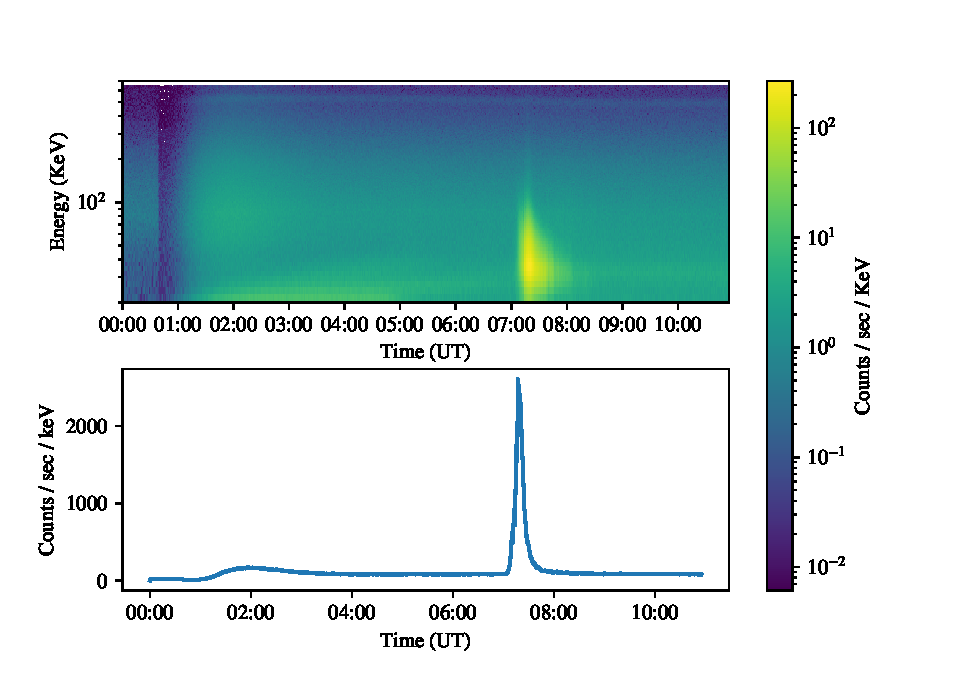
\includegraphics[width=1.0\textwidth]{figures/chapter_5/epex_spectrogram/epex_spectrogram__with_cps_cbar-2}
    \caption{EPEX X-ray spectrometer data in spectrogram form. The precipitation event was observed at 07:00 UTC. The total counts per second are shown below the spectrogram as a function of time.}
    \label{epex_event_spectrogram}
\end{figure}

A background-subtracted spectrum of the precipitation event is shown, along with the reconstruction using the techniques of Chapter 4, in Figure~\ref{epex_fit_comparison}. The retrieved precipitating electron spectrum is shown in Figure~\ref{epex_tk_inv}. It was generated using second-order Tikhonov regularization with left and right diagonal preconditioning and a positivity constraint. The X-ray spectrum data from 70 to 500 keV were fit. The retrieved electron spectrum has a very mono-energetic structure at approximately 80 keV. The model agrees well with the data, unlike the result from the $\text{ABOVE}^2$ event, because this detector was flown in a refurbished and undamaged state. The total precipitating electron flux is estimated by the model as $4.8\times 10^8$ electrons $\text{cm}^2$ / second. This was a very bright event which was well-defined in time and energy. The low value of $\alpha = 3.5\times10^3$ (compared to the $\text{ABOVE}^2$ event) suggested by cross-validation indicates that a good fit to the data was found by the reconstruction algorithms without requiring intense reconditioning of the problem. This is consistent with the fact that this bright event has a very high signal to noise ratio in the background subtracted data. This event can serve as an example of the usefulness of the regularization techniques in analyzing X-ray data. The regularized model in Figure~\ref{epex_fit_comparison} shows better agreement with the data than either the best exponential or monoenergetic fits. The reduced $\chi ^2$ statistics for the monoenergetic and exponential fits are 0.53 and 58.0, respectively. The reduced $\chi ^2$ for the regularized model is 0.75. This indicates that the exponential fit is a bad description of the X-ray data set for this event. The monoenergetic fit is better, but the regularized solution is best, having a reduced $\chi ^2$ statistic closest to 1.0. The strength of the regularization methods, combined with cross-validation, is that, with mild assumptions, we can a model-independent characteristic energy and width of the electron distribution. 

\begin{figure}[p]
    \centering
    \includegraphics[width=1.0\textwidth]{figures/chapter_5/epex_fit_comparison/epex_fit_comparison2.pdf}
    \caption{Background-subtracted X-ray event measured by the EPEX spectrometer. The model fit using Tikhonov regularization is shown overlaid.}
    \label{epex_fit_comparison}
\end{figure}

\begin{figure}[p]
    \centering
    \includegraphics[width=1.0\textwidth]{figures/chapter_5/epex_tk_inv/epex_tk_inv2.pdf}
    \caption{Precipitating electron spectrum retrieved from EPEX X-ray data using the techniques of Chapter 4. The required value for $\alpha$ is low and well-defined through cross-validation.}
    \label{epex_tk_inv}
\end{figure}

\section{The BARREL Campaign}

I examine one flight from the NASA BARREL balloon campaign, which occurred during 2014. This flight was launched with an X-ray spectrometer similar to those flown on the EPEX and  $\text{ABOVE}^2$ campaigns, and recorded an electron precipitation event while magnetically local to an orbiting spacecraft (Van Allen Probe B), which provides conjugate measurements of energetic electrons via the MAGEIS instrument. This flight was analyzed by~\citet{Halford2015}, who determined that the precipitation event occurred in the aftermath of an ICME (interplanetary coronal mass ejection) shock. Since the BARREL balloon was airborne and recoding data while the spacecraft was on the same approximate L-shell, \citet{Halford2015} could complete an ``end-to-end'' study of the recorded precipitation event, from creation, to detection by an RBSP spacecraft, to the precipitation in the atmosphere and resulting creation of X-ray radiation detected by the balloon. We will analyze the event measured by the balloon in this section.

A spectrogram of the event observed by~\citet{Halford2015} is shown in Figure~\ref{barrel_spectrogram}. This is a very low intensity event, but it occurs over a time period of tens of minutes. We will use an average spectrum taken over the event time range. The background-subtracted spectrum of the event, and the best-fit model spectrum is shown in Figure~\ref{barrel_fit_comparison.}. Finally, the retrieved electron spectrum is shown in Figure~\ref{barrel_tk_inv}. The retrieved electron spectrum has two main components, a distribution at around 250 keV, and a smaller high energy component at around 600 to 700 keV. The significance of the high energy component is not clear, since the X-ray spectrum has a noise floor which begins at approximately 200 keV. 

\begin{figure}[p]
    \centering
    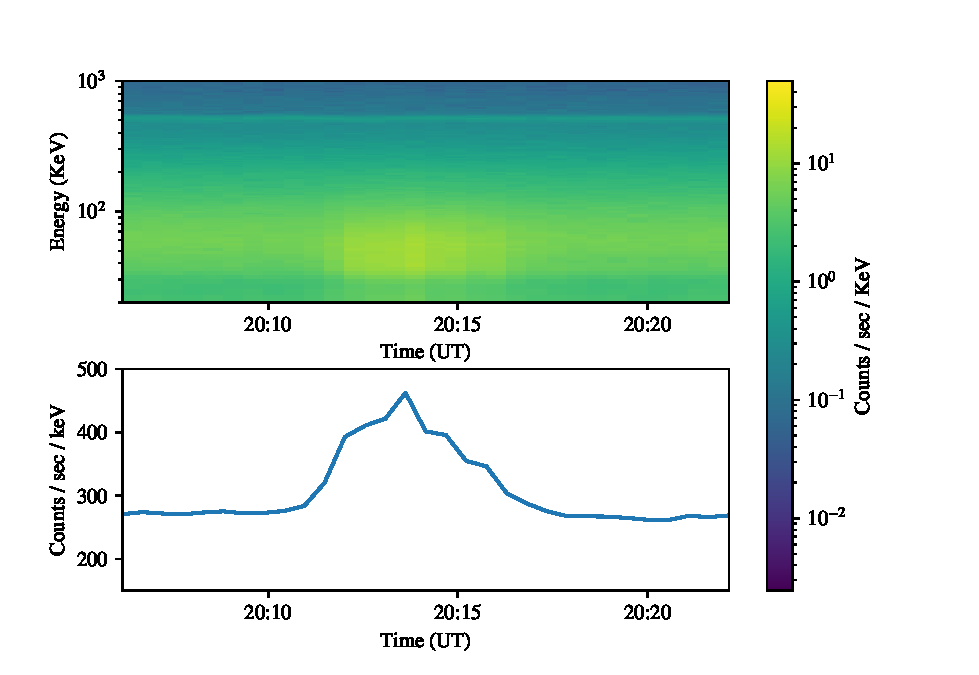
\includegraphics[width=1.0\textwidth]{figures/chapter_5/barrel_spectrogram/barrel_spectrogram}
    \caption{Spectrogram and raw count rates of the event measured by BARREL and studied by~\citet{Halford2015}.}
    \label{barrel_spectrogram}
\end{figure}

\begin{figure}[p]
    \centering
    \includegraphics[width=1.0\textwidth]{figures/chapter_5/barrel_fit_comparison/barrel_fit_comparison}
    \caption{Background-subtracted X-ray event measured by the BARREL spectrometer. The model fit using Tikhonov regularization is shown overlaid.}
    \label{barrel_fit_comparison}
\end{figure}

\begin{figure}[p]
    \centering
    \includegraphics[width=1.0\textwidth]{figures/chapter_5/barrel_tk_inv/barrel_tk_inv}
    \caption{Precipitating electron spectrum retrieved from BARREL X-ray data using the tfechniques of Chapter 4. The required value for $\alpha$ is approximately $5\times10^2$.}
    \label{barrel_tk_inv_2}
\end{figure}

\subsection{Energy Selective Scattering}

As a validation of the inversion method, the electron spectrum can be compared with in-situ measurements of the corresponding electron flux measured by the satellite in the magnetosphere. The in-situ data provides a limit on the precipitating electron flux, which is the product of the available flux and the scattering efficiency. A subset of the flux measured by the satellite will precipitate into the atmosphere.  

Spacecraft measurements of energetic electrons do not generally resolve the population within the loss cone.  We show that the techniques developed in Chapter~4 can be applied to infer this energy range from balloon measurements, by building on an analysis published by~\citet{Halford2015}. \cite{Halford2015} reported on an energetic electron precipitation event that happened while one of the Van Allen Probe B was at a similar L-value and close in MLT with a BARREL balloon 2L that measured the resulting X-ray spectrum. Their analysis provides an end-to-end picture that describes the scattering processes which drove the event, and the measurable impact it made on the atmosphere.  

The Van Allen Probes are a pair of orbiting spacecraft which carry instruments to understand electron acceleration in the radiation belts. The Magnetic Electron Ion Spectrometer (MAGEIS) instruments are magnetic spectrometers that provide in-situ measurements of the energies, angular distributions, and differential fluxes of electrons in the radiation belts~\cite{Blake2013,Spence2014}. There are four magnetic spectrometers on each spacecraft, each designed for a specific energy range. Electrons enter each instrument through a collimator and are deflected to a pixelated detector surface by a uniform magnetic field. We will use the pitch angle resolved, background-subtracted differential energy fluxes provided by the Energetic Particle, Composition, and Thermal Plasma (RBSP-ECT) investigation~\cite{Spence2013}.

A key assumption that must be made in the analysis of the precipitation event from~\cite{Halford2015} is that the available MAGEIS data in the lowest (approx. 8 degree)  pitch angle bin represents the energy distribution of electrons that are scattered into the loss cone. This is because MAGEIS does not resolve fluxes within the loss cone. The assumption is that the electron spectrum in the loss cone is the same as the electron spectrum in the lowest pitch angle bin, except that it has undergone a scattering process which selects for a range of electron energies. but leaves the rest of the spectrum unaltered. ~\cite{Thorne2010} uses quasi-linear theory and satellite data to show that chorus waves lead to rapid pitch angle scattering over a narrow pitch angle range near the loss cone for electrons from 100 eV to a few keV. 

 \cite{Halford2015} apply exponential and mono energetic fits to the measured X-ray data, and also compared with the energy spectra observed near the loss cone from Van-Allen Probe B MagEIS data which was at a similar L-value and close in MLT to BARREL payload 2L (see Figure 4 in \cite{Halford2015}). The best fit to the observed X-ray spectra was found when using the observed energy spectra from Van Allen Probe B. The agreement reveals that the measured event does contain enough information to distinguish between electron beams with zero width (mono-energetic), and beams which extend to the highest modelled energy (exponential). We use this event as a test of the regularization method to see how much more information about the scattered electron spectrum it can extract. In particular, under the assumption that the scattering processes responsible for the observed precipitation select an energy range from the magnetically conjugate Van-Allen Probe measured electron spectrum, we evaluate if that energy range can be determined from the X-ray data. 

The comparison of mono-energetic and exponential fits to the balloon X-ray spectrum done by~\cite{Halford2015} is reproduced in Figure~\ref{barrel_electron_fit_comparison}. We apply the constrained second-order regularization technique to obtain a model electron spectrum. The X-ray spectrum predicted to result from this retrieved spectrum is plotted with the measured X-ray data, and shows closer agreement with the BARREL spectrum than the best fits that can be produced by assuming the mono-energetic or exponential forms. 

\begin{figure}[p]
    \centering
    \includegraphics[width=1.0\textwidth]{figures/chapter_5/barrel_electron_fit_comparison/barrel_fit_comparison_2}
    \caption{Mono-energetic and exponential fits to the BARREL event from ~\cite{Halford2015}, with the fit obtained by applying the techniques developed in Chapter~4 (preconditioned, constrained second-order Tikhonov regularization using cross-validation). The total electron flux for the regularized model is found to be $1.6 \times 10^6 \mbox{electrons}/\mbox{cm}^2/\mbox{sec}$.}
    \label{barrel_electron_fit_comparison}
\end{figure}

Data from the RBSP MAGEIS instrument used in the analysis of the ~\cite{Halford2015} event is shown in Figure~\ref{mageis_spectrum}. Under the assumption of strong scattering, with a full loss cone. The topside electron flux from a spacecraft in magnetic conjunction with a given location on Earth is given as $F\approx (B_{i}/B_{top}) J_{top} \Delta \Omega$ ~\citep{kasahara2018}. $B_{i}$ and $B_{top}$ are the magnetic field strengths at the precipitation point and spacecraft, and $J_{top}$ is the electron flux at the spacecraft. $\Delta \Omega$ is the width of the loss cone at the spacecraft. 

This estimate requires the assumption that the electrons measured in the lowest pitch angle bin of the MAGEIS data (approximately 8 degrees) represent the energy spectrum of electrons in the loss cone. The radio of solid angles subtended by 8 degrees and 2.5 degrees is $10.22$. The ratio of magnetic field strengths at the MAGEIS instrument and at the balloon is approximately $150 \text{nT}/55000{nT} = 366.6$. Using this, the expected precipitating electron spectrum based on the MAGEIS data is shown in Figure~\ref{mageis_spectrum}. The inferred precipitating electron spectrum based on the regularized solution from the balloon data is shown in the same units. 

\begin{figure}[p]
    \centering
    \includegraphics[width=1.0\textwidth]{figures/chapter_5/mageis_spectrum/mageis_spectrum_2}
    \caption{Expected precipitating electron spectrum as measured by RBSP-B MAGEIS and model spectrum generated from measured balloon data using Tikhonov regularization.}
    \label{mageis_spectrum}
\end{figure}

The precipitating spectrum inferred from the measured balloon data is subset to the spectrum predicted to precipitate from the MAGEIS data. This is an expected result, since the electron population in the loss cone at the spacecraft represents a total available flux which can precipitate, while the balloon spectrum represents the actual population that did precipitate and impact the atmosphere. This supports the value of balloon measurements of precipitating electron spectra. The shape of the energy spectrum obtained from the balloon data is different than the population measured by the MAGEIS instrument on the spacecraft. The determination of this shape using Tikhonov regularization represents additional information which is available in the balloon X-ray data, which is not retrieved when fitting assumed forms for the precipitating electron spectrum. The information carried by the shape of the precipitating spectrum also represents information about the scattering processes responsible for the precipitation, since they are energy dependent. 







\chapter{Conclusions}

\section{The Inverse Problem}

The primary question addressed by this thesis is how much information can reasonably be expected to be obtained from balloon measurements of X-ray spectra. The key results for the analysis methods are as follows:

\begin{itemize}
\item When accompanied by an accurate forward model of the expected instrument response given a precipitating electron spectrum, the electron spectrum can be recovered provided that the measurement noise is low enough. 
\item The required statistical purity in the measured X-ray spectrum depends on the shape of the particular spectrum being recovered, and the amount of detail sought in the solution.
\item Preconditioning techniques such as diagonal scaling improve the condition of the inverse problem with no additional assumptions or bias.
\item Biased estimators, such as truncated singular value decomposition, or Tikhonov regularization, can be applied to the to the inverse problem to make it tractable in realistic simulations and actual experiments. 
\item The application of cross-validation methods provides a way to balance the required stability of the solution against the inherent ill-conditioning of the problem, and is capable of selecting regularization parameters which represent the available information in the data without requiring heuristic arguments or detailed assumptions on the form of the output. 
\end{itemize}

These conclusions, when taken together, form a picture of the X-ray inversion problem that is quite different than what is being currently used in experiments. As discussed in Chapter 4, the ill-conditioned inverse problem needs to be addressed to obtain meaningful results. The conventional approach of assuming a particular functional form for the model electron spectrum solves the ill-conditioning by reducing the parameter space of the model. The analysis subsequently uses the well-known $\chi^2$ tests to select an optimal fit and produce an error estimate for that fit. This approach, favoured for its relative simplicity and ability to produce an error estimate, necessarily gives a misleading solution. The reason is that the uncertainty presented by the ill-conditioning of the problem, which results in the vast majority of the uncertainty in the solution, is effectively ``swept under the rug'' and contained in the assumption on the model function chosen for the solution. The remaining error analysis is trivially based on counting statistics and cannot be used to identify between different model spectra, except when significant a-priori information about the precipitating spectrum is known. 

This perspective assumes that very little useful information can be obtained from X-ray measurements. This thesis offers an alternative picture: instead of reducing the information extracted from the data to fit the analysis methods, we adapt the analysis based on what can be determined from the data in a given scenario. This picture is much more optimistic, but critically, it isn't unrealistic. The linearity of the forward problem, combined with the widespread availability of sophisticated particle transport software, makes constructing an accurate representation of the balloon experiments possible. Then, different frameworks for solving the inverse problem can be tried and compared using simulated data. We have found that some relatively simple linear algebra can be used to relieve most of the ill-conditioning of the problem, without loss of generality, but that the transformed problem still requires the use of a biased estimator to give useful, general, results in realistic situations. 

Tikhonov regularization, which is a specific form of the general techniques which modify the singular value spectra of the response matrix of the forward problem, provides a way to continuously adjust the effective dimensionality of the solution, and therefore, the amount of information solved for. Combining this parameterization with cross-validation allows for the optimized selection  of the amount of information contained in the solution, so that it neither underfits, no overfits, the available data. In particular, second-order Tikhonov regularization effectively blurs the detail in the represented solution to match the data, and requires no general assumptions on the shape of the model spectrum. Tikhonov regularization can be done using constraints which further reduce the parameter space of the problem at no additional cost. Particularly, we have found that a simple positivity constraint reduces the dispersion in model spectra. This ensemble of methods is modular - in the sense that additional constraints may be added, without additional loss of generality, if any a-priori information about the precipitating spectrum is known, for example, if magnetically local spacecraft measurements are available.

The primary cost of the use of biased estimators is that they force the mismatch between the information in the input and output of the ill-conditioned problem out in the open - we now have to handle it, and its consequences. This can be taken as a more honest view of the inverse problem in general. While the techniques in Chapter~4 provide strong results when applied to synthetic data, what they cannot do, is provide standard error bars on the shape of the output spectrum. This is because poisson statistics and their simple interpretation no longer apply in the same sense under biased estimators. Statisticians have said that the determination of meaningful error estimates for this kind of problem is one of the frontiers of their research. This places it well outside the scope of this thesis to address, and at the time of writing, only preliminary results exist, and none in the less abstract form needed for practical application to this particular problem. 

The key point is this: it is better to have the fundamental lack of information that causes the ill-conditioning of the inverse problem accounted for in some way, than to conceal it behind an assumption which cannot be justified in most experiments. By honestly attempting to, at least heuristically, account for the amount of information available in a given dataset and in a particular situation, we can learn more than by the misapplication of simple, but tractable, analysis methods.

A secondary conclusion comes from the necessity of a forward model of the precipitation process. The inverse problem, owing to its ill-conditioning, is highly sensitive to both noise, and bias, in the input data. It follows that the accuracy and precision of the forward model used to represent the problem must be high enough not to significantly affect tests on simulated data. The exact instrument response plays a key role in the forward model, and is something that cannot be adequately determined through simulation alone. Lab measurements against known X-ray spectra are required for every different experiment. These are not always easy to accomplish, owing to the somewhat random, and discrete, X-ray peaks produced by commonly available radioactive sources. Further, the instrument response needs to be well-approximated as linear with regards to energy, in order for it to be applied to the linear framework developed to address the inverse problem. The critical simplification made in Chapter~3 was that the instrument response in counts to a monochromatic beam of X-ray photons could be represented using a Green's function approach. Additionally, a large simplification of the forward problem was obtained by essentially ignoring the angular distribution of the precipitating electrons. In this sense it made the problem separable, and reduced the inverse problem to one dimension in energy only.

The environment surrounding the particular detector will need to be simulated in the forward model if it changes significantly between lab testing and installation in a balloon. Balloon experiments are hosted in insulated containers, which are usually surrounded by other flight components, some of which can interact with natural radiation in significant ways. None of this is insurmountable, but needs to be made explicit in light of the primary conclusions. All of the work in Chapter~4 and the subsequent analysis of experimental data applies because the forward model of the experiment was available and verifiable against lab data. Future experiments, even ones flown with changes only to the support systems and flight hardware, rather than instrument itself, will need to re-evaluate the conclusions of Chapter 4, based on the altered forward model of the problem. This could be seen as a lack of generality. It is instead an acknowledgement that the inverse problem is fragile to small changes in the input data and response matrix. This is not as significant of a problem when artificially suppressed by strong assumptions on the output. 

\section{Application to Experimental Data}

When applied to the available body of experimental data (U of C balloon flights and the BARREL campaign), application of the analysis techniques we have developed support the following conclusions:

\begin{itemize}
\item X-ray data obtained from sodium iodide scintillation detectors is sufficient to determine useful information about the precipitating electron spectrum, including the overall electron flux and approximate energy distribution. 
\item In the case of the precipitation event recorded by a balloon when magnetically local spacecraft measurements of the electron spectrum were available, the data can be used to infer a spectrum compatible with the spacecraft measurements, in the sense that the retrieved energy spectrum produces approximately the precipitating electron flux that would be expected based on the spacecraft measurements under the strong scattering assumption with a full loss cone.
\item When the instrument is not performing according to the forward model, as in the U of C balloon flight where it was damaged, our analysis of the data shows a clear problem with the fit. 
\end{itemize}


The first conclusion has been known since the earliest balloon experiments equipped with X-ray detectors were flown. The questions that have persisted over the subsequent decades have all hinged on the interpretation of the measured data, and the amount of information that can be obtained from them. The primary contribution of this thesis to the problem is to demonstrate  that the amount of information available is well-represented as a continuous function of the bias and noise level of the particular experiment flown. This function can be parameterized as a one dimensional optimization, which prevents the introduction of experimenter bias. 

The second conclusion relies on available magnetically connected satellite measurements to the balloon measuring the precipitating spectrum. These occurrences are subset to the available balloon data, and owing to the logistical challenges of timing balloon release against spacecraft orbits, and the expense of balloon flights in general, are not common. The event analysed in Chapter~5 from ~\citet{Halford2015} provides a picture that extends from the trapped population in the radiation belts, through scattering and finally precipitation to the atmosphere and detection by the balloon spectrometer. The measured spectrum at the spacecraft and the spectrum measured by the balloon are not the same - in general, the precipitating population will be subset to the population measured by the spacecraft, and the population will undergo a largely unknown scattering process prior to precipitation. Having measurements of the population from the spacecraft and the balloon does, however, permit a more detailed picture of the end-to-end process to be created. Under the assumption of strong scattering and a full loss cone, and the assumption that the electron population in the lowest pitch angle bin resolved by the spacecraft represents the population in the loss cone, then the precipitating electrons should be subset. Under the additional assumption that the scattering processes responsible for the precipitation are energy selective (which is reasonable, based on the wave-particle dynamics explored in Chapter~2), the balloon spectrum represents the population that was scattered into the loss cone. Since the analysis techniques of Chapter~4 allow the determination of the energy spectrum and total flux of the precipitating population, we have an end-to-end picture of the scattering and precipitation process. Given an estimate of the energy range of the precipitating electrons, the work done by~\citet{kasahara2018} allows the estimation of a precipitating electron flux from the spacecraft data. The results were consistent. Although this is not a direct comparison between two independent sources of data, the overlapping data available between the balloon and the satellite are consistent, which suggests that, given more balloon-satellite conjunctions and measurements, we could show experimentally that the balloon data are sufficient to quantify the precipitating spectrum.

\section{Future Work}

\subsection{Simulations and Models}

To be useful to balloon experiments, the analysis in chapters 3 and 4 needs to be expanded to include different detector designs and specifications. In this thesis, we have demonstrated the effectiveness of one particular detector design, in one experimental setting. Next generation solid state and plastic scintillators have different properties than the sodium iodide crystals used in this work, and their analysis will depend on an accurate representation and simulation. The question of whether a different detector design could be more effective at providing data that solves the inverse problem is so far, unanswered. If differently designed detectors have more complex responses to X-ray photons, which require a different mathematical representation, then much of the work done in Chapter~4 will need to change to account for this. It is not known whether the preconditioning and regularization techniques will still provide useful results given a different detector model.

The analysis techniques developed in Chapter~4 assume an even sampling of energy spectra, using constant-width rectangular bins. This is likely not optimal, and it may be beneficial to increase the effective bin width, and lower the resolution of represented spectra, with increasing energy. There is no reason that this alteration of energy resolution needs to be linear. Accounting for the fact that the lower recorded counts at high energies should have a lower encoded resolution is standard in detector design, and it should be explored for potential benefit in the analysis as well.

The main piece of knowledge that the analysis we have developed does not provide is an estimate on the error in the developed solution. This is a current topic of research in applied statistics, and there are no simple ways to add this function to the analysis method. There are theoretical methods to provide estimates of the spread of confidence intervals over subsequent measurements of the same spectrum, but this is information that is generally not available experimentally. Once a precipitation event occurs, recording the same event multiple times isn't possible. Recent work on the generation of meaningful confidence intervals for biased estimators is ongoing. It may be that a practical method is found, and can then applied to the X-ray inversion problem. 

One actionable method which could be applied today, is the computation  through the forward model of many different prototype functions, and their subsequent inversion under specific assumptions on the noise and bias of the instrument in use. Given a rough form for the retrieved spectrum, using the techniques in Chapter~4, the behaviour of changes to counting statistics on the input data could be roughly quantified through monte-carlo simulations. This will depend on specific knowledge of the detector being used for a given experiment. There are no general results at present. 

The simplification obtained by ignoring the angular spectrum of the precipitating electrons also results in a loss of information that can be obtained from the data. Future detectors which have angular resolution could, in principle, be used to obtain data on the location, size, and  shape of patches of precipitating electrons. This anaylsis would require moving from a 1 dimensional representation of the inverse problem to a 2 dimensional model. Based on the computation required to generate the forward model in Chapter~3, which was done for one assumed angular distribution, the required computational resources will be large, and possibly impractical without a significant reparameterization of the model. Based on the current analysis, three dimensional histograms would need to be generated for every possible input. Hundreds of hours of computer time on significantly parallel machines was required to form the model used in this thesis, so such an approach would likely not be sucessful. What may work is the refactoring of the forward model into a set of different basis functions, such as spherical harmonics, or perhaps others, which are orthogonal, or sufficiently orthogonal to not make the inverse problem impossible.The design of detectors which can resolve angular distributions in incoming X-rays from balloons will need to take into account the ill-conditioning of the one dimensional problem. Their output will need to be simulated, and tests on synthetic data carried out, to see  how much information can be obtained from them. 

\subsection{Experimental Data}

Despite successful campaigns of zero-pressure balloons flown over months, and multiple flights of opportunity taken when satellite conjunctions are available and space weather is favorable to precipitation events, there is still a great need for more data which can be compared between balloons and spacecraft. Tests based on synthetic data alone are not sufficient to fully validate the method. For this to happen, we need pitch-angle resolved measurements of precipitating electrons in space, which are magnetically conjugate to the balloon measurements. If an expected precipitating spectrum could be detemined, free from strong assumptions on the scattering processes responsible, then a more direct comparison with the balloon data would be possible. The techniques developed in this thesis also permit the analysis of X-ray data for comparatively low intensity precipitation events when the counting statistics available in the recorded data are not very pure. Given the large dataset of the BARREL balloon flights, there are certainly events available which can be analysed, that have not yet. 

The next generation of instrumented balloons may greatly increase the depth of the available data. Work done at the University of Calgary to develop rapidly deployable, low cost, long duration balloons has shown promising initial results. When combined with lightweight solid-state detectors, and flights which permit recovery operations, it is hoped that flights of opportunity can be accomplished as active space weather conditions occur. The reduced cost and risk of this type of flight may make it an attractive platform on which to run X-ray measurement experiments. 






\newcommand{\newblock}{}
\bibliographystyle{plain}
\bibliography{library}

%\appendix
%\include{appendix_1}
\end{document}
